%!TEX options = --shell-escape
\documentclass[cn,pad,twocol]{elegantbook}
\usepackage{array}
\usepackage{xpinyin}
\usepackage{fancyhdr}
\usepackage{bookmark}
\pagestyle{fancy}
\usepackage[noheader]{gitver}
\usepackage{hyperref}
\hypersetup{
	pdftitle={北園習箫谱},
    pdfauthor={青箫散人},
}

\title{北園習箫谱}
\author{青箫散人}
\date{\zhtoday}
\cover{cover21}
\logo{monk.png}
\extrainfo{清籁远\xpinyin*{喑}喑,秦楼夜思深。碧空人已去,沧海凤难寻。\\杳妙和云绝,依微向水沉。还将九成意,高阁伫芳音。}
\version{\gitVer}
\fancyfoot[C]{明月如霜,青箫独吟,小桥清溪枯柳。杯黄酒,又见纤纤酥手舞彩袖。}

\begin{document}
\maketitle
\frontmatter
\tableofcontents
\mainmatter

\chapter{箫的来历}
\paragraph*{箫,形声。字从竹从肃,肃亦声。“肃”本义为“千针万孔”,转义为“风声尖锐地漫天呼啸”。“竹”与“肃”联合起来表示“一种模拟风声漫天尖锐呼啸的竹制吹奏乐器”。本义:一种模拟风吹声的竹乐器。箫是中国古老的吹管乐器,特征为单管、竖吹、开管、边棱音发声\footnote{袁静芳,名族乐器,高等教育出版社 2004 ISBN7040150026}。}
\begin{center}
    \vfill
    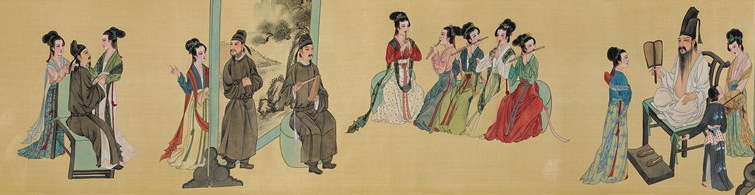
\includegraphics[width=\textwidth]{cover8}
\end{center}

\paragraph*{箫源于远古时期的骨哨,新石器时代开始以竹制作。历史上亦称为笛,在秦汉至唐,箫是指编管的排箫。唐以后方专指竖吹之笛。“横吹笛子竖吹箫”,即笛箫之间最基本的差别。箫历史悠久,音色圆润轻柔,幽静典雅,适于独奏和重奏。} 
\paragraph*{早在《尚书·益稷》中记载有“\xpinyin*{箫韶九成,凤凰来仪}。”当因韶乐伴奏乐器以箫(当时为排箫)为主而有此称。箫在汉代时称为“\xpinyin*{篴}”、“竖篴”。西晋乐工列和、中书监荀勖所改革的笛为6 孔(前5、后1),其形制与今天的箫已非常相似了。东晋的桓伊,擅长音乐,他有一支蔡邕的柯亭笛(箫),是江南数第一的吹箫名手,地位和声望都已很高。他曾为素不相识的王徽之吹奏过三段乐曲,在历史上被传为佳话。}
\paragraph*{魏晋南北朝时,箫已用于独奏、合奏,并在伴奏相和歌的乐队中使用。清代,箫的形制完全一样。清《律吕正义后编》记载:“明时乃直曰箫,不复有竖篴。今箫长一尺八寸弱,从上口吹,有后出孔;笛横吹,无后出孔。”}
\paragraph*{当代箫有三种,分别是琴箫,洞箫和南箫。三种箫最大的区别是管径,音色稍有差异。琴箫最为细腻,南箫在稍显粗狂豪放,洞箫介于二者之间,玩转悠然。日本的尺八,是由唐尺八传到日本。后经过多年改革,并结合日本本土文化形成的日本民族乐器,音色沧桑悲凉。实际上,他们的音色差别并不大,主要是乐曲本身的特色带来的感觉。}
\paragraph*{形制上,箫有粗短型和细长型。管体较粗而短之箫,为传统古洞箫,或称南箫\footnote{祁台颖,林品义等 四个年轻孩子与一百种市井职人相遇的故事 远流出版社 2010 ISBN9789573267294}。以南管箫为代表,桂竹、孟宗竹、石竹制成。前5空,后一空,十目九节,吹口为V型。音色浑厚深沉,吹奏时双臂抬成凤凰展翅之势。细长型\footnote{傅湘仙 尺八古琴考 上海音乐学院出版社 2005 ISBN7806921680}管体较细而长。如琴箫,又称北箫。多以紫竹制成,体型细小,管身细长而音量较小。}
\paragraph*{切口,分为U口、V口和唐口。唐口则是尺八的开口,外切。}
\chapter{指法图}
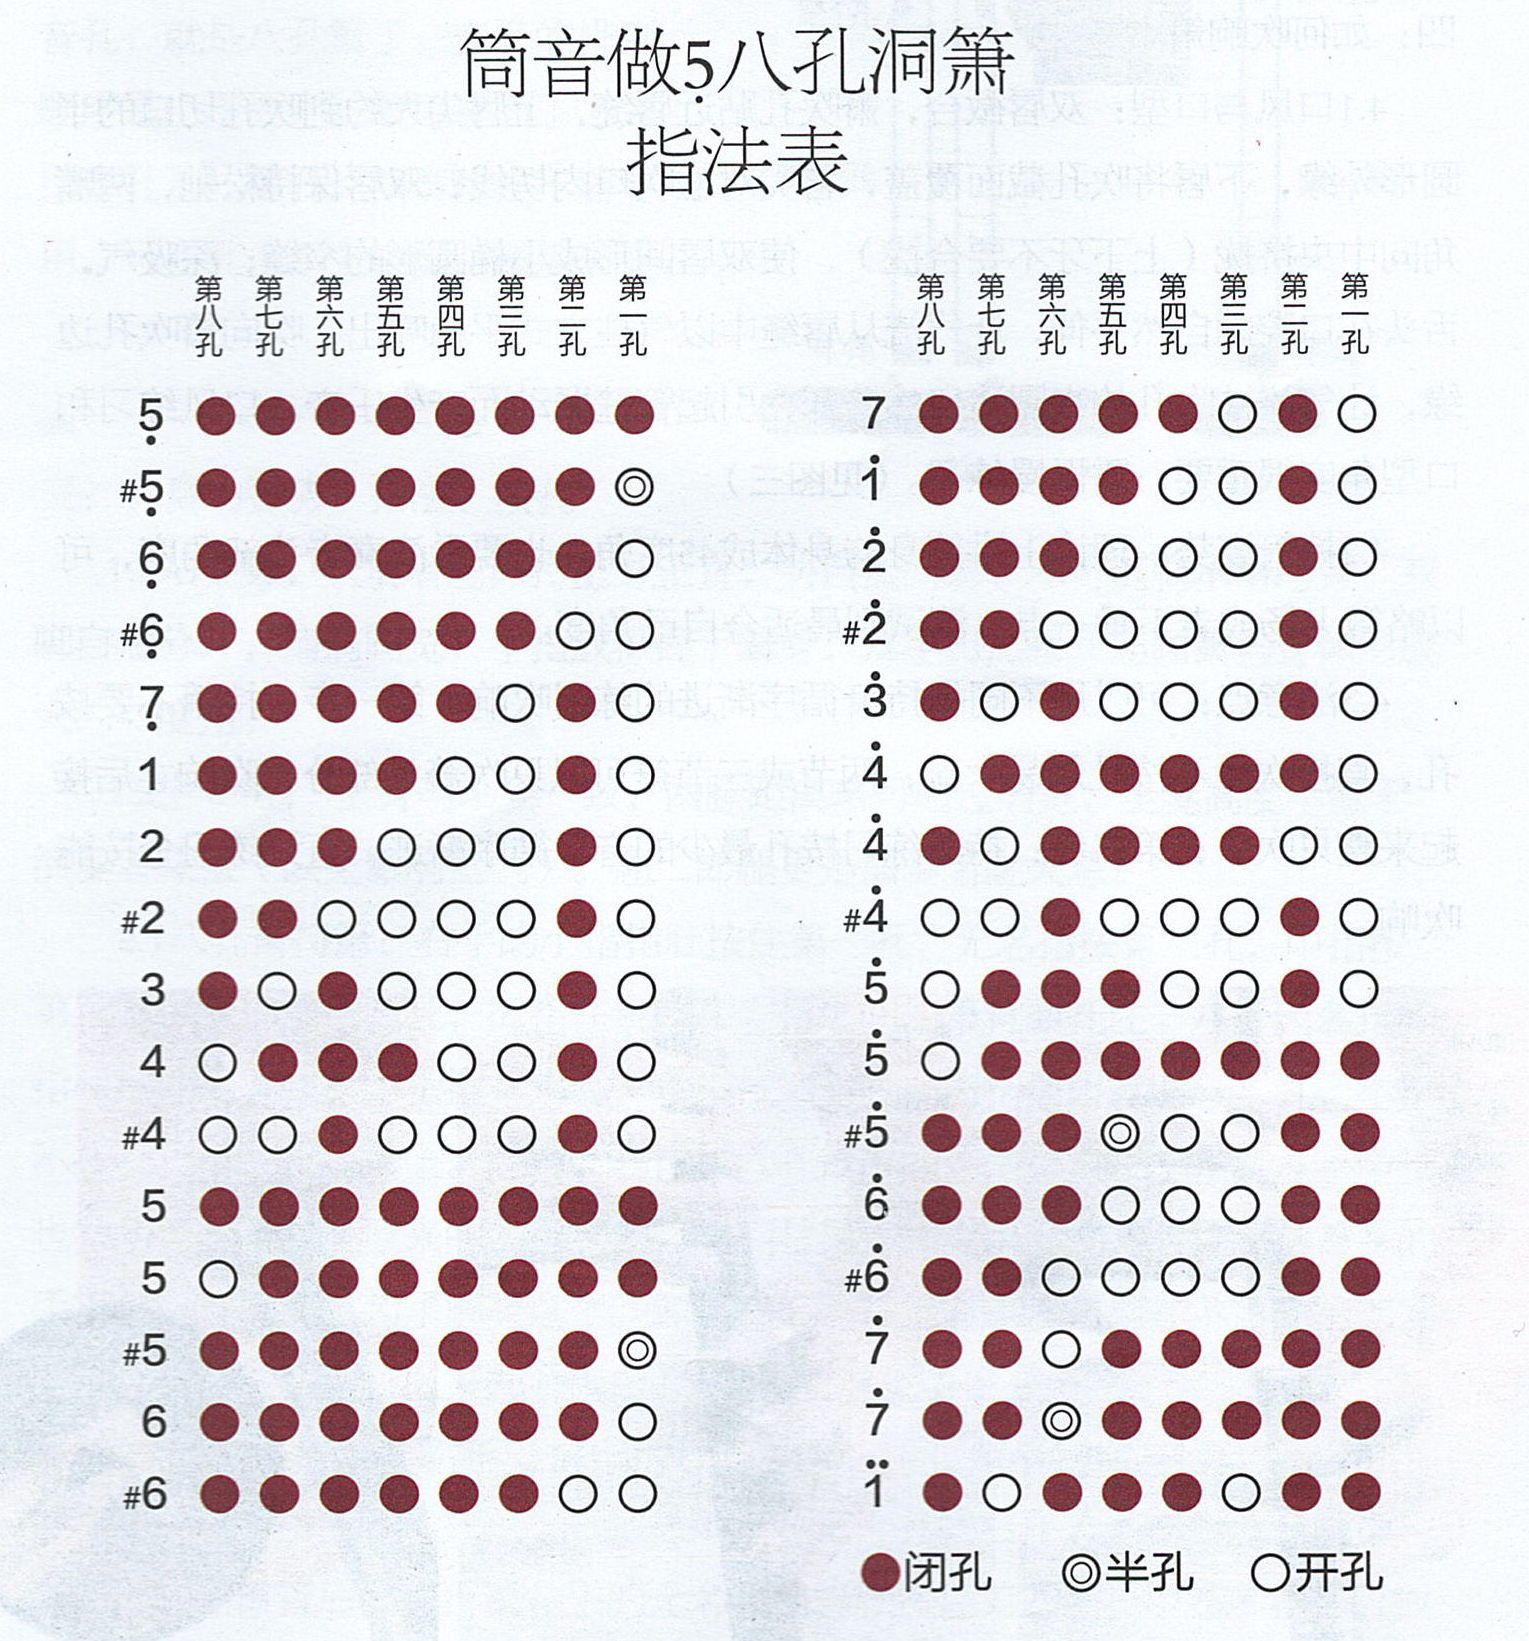
\includegraphics[width=0.93\textwidth]{dongxiao/Scan.jpeg}
\chapter{基礎谱}
\section{筒音作5}
\begin{center}
	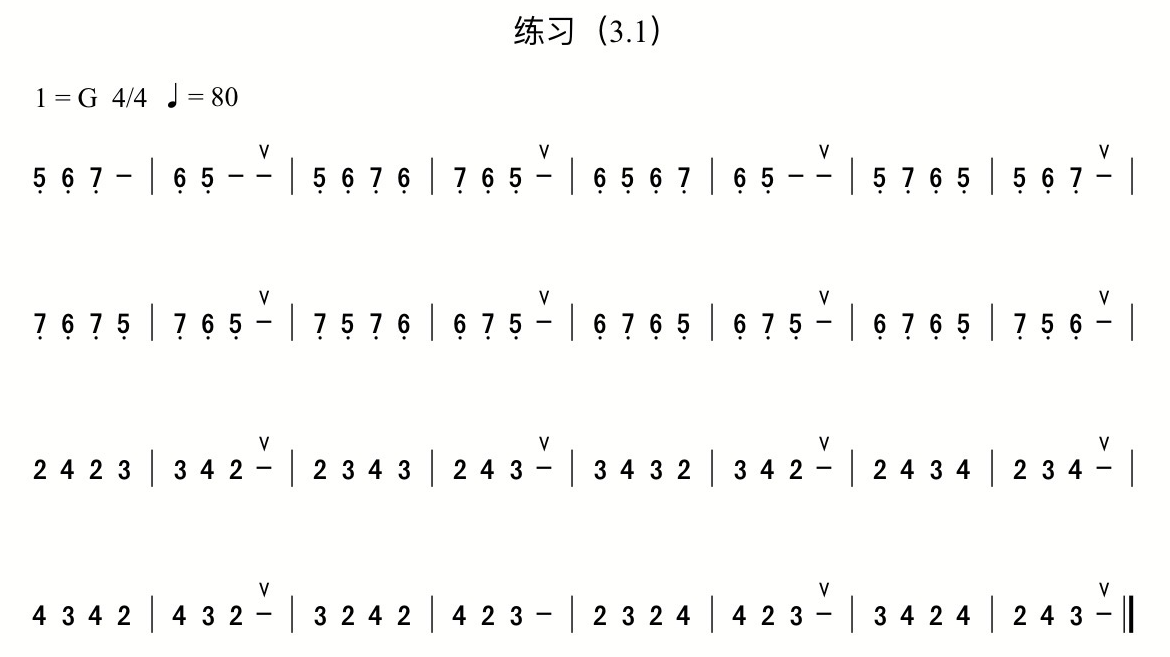
\includegraphics[width=\textwidth]{dongxiao/20200419-练习3.1.png}
\end{center}
\section{筒音作2}
	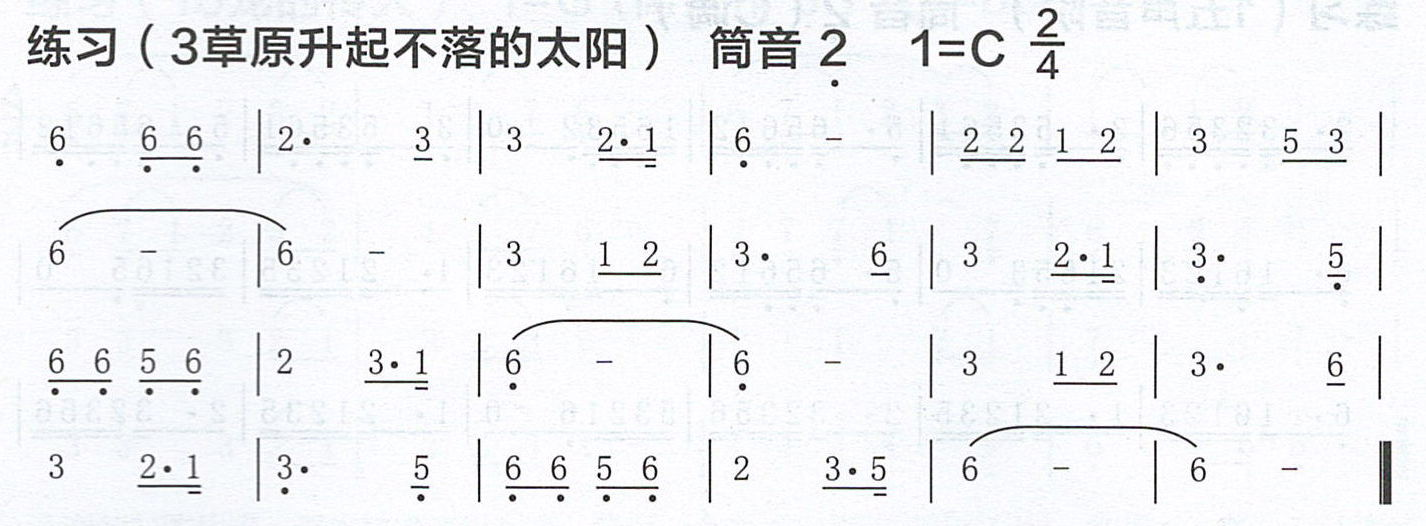
\includegraphics[width=\textwidth]{dongxiao/Scan 6.jpeg}

\chapter{首选}
\section{世上只有媽媽好}        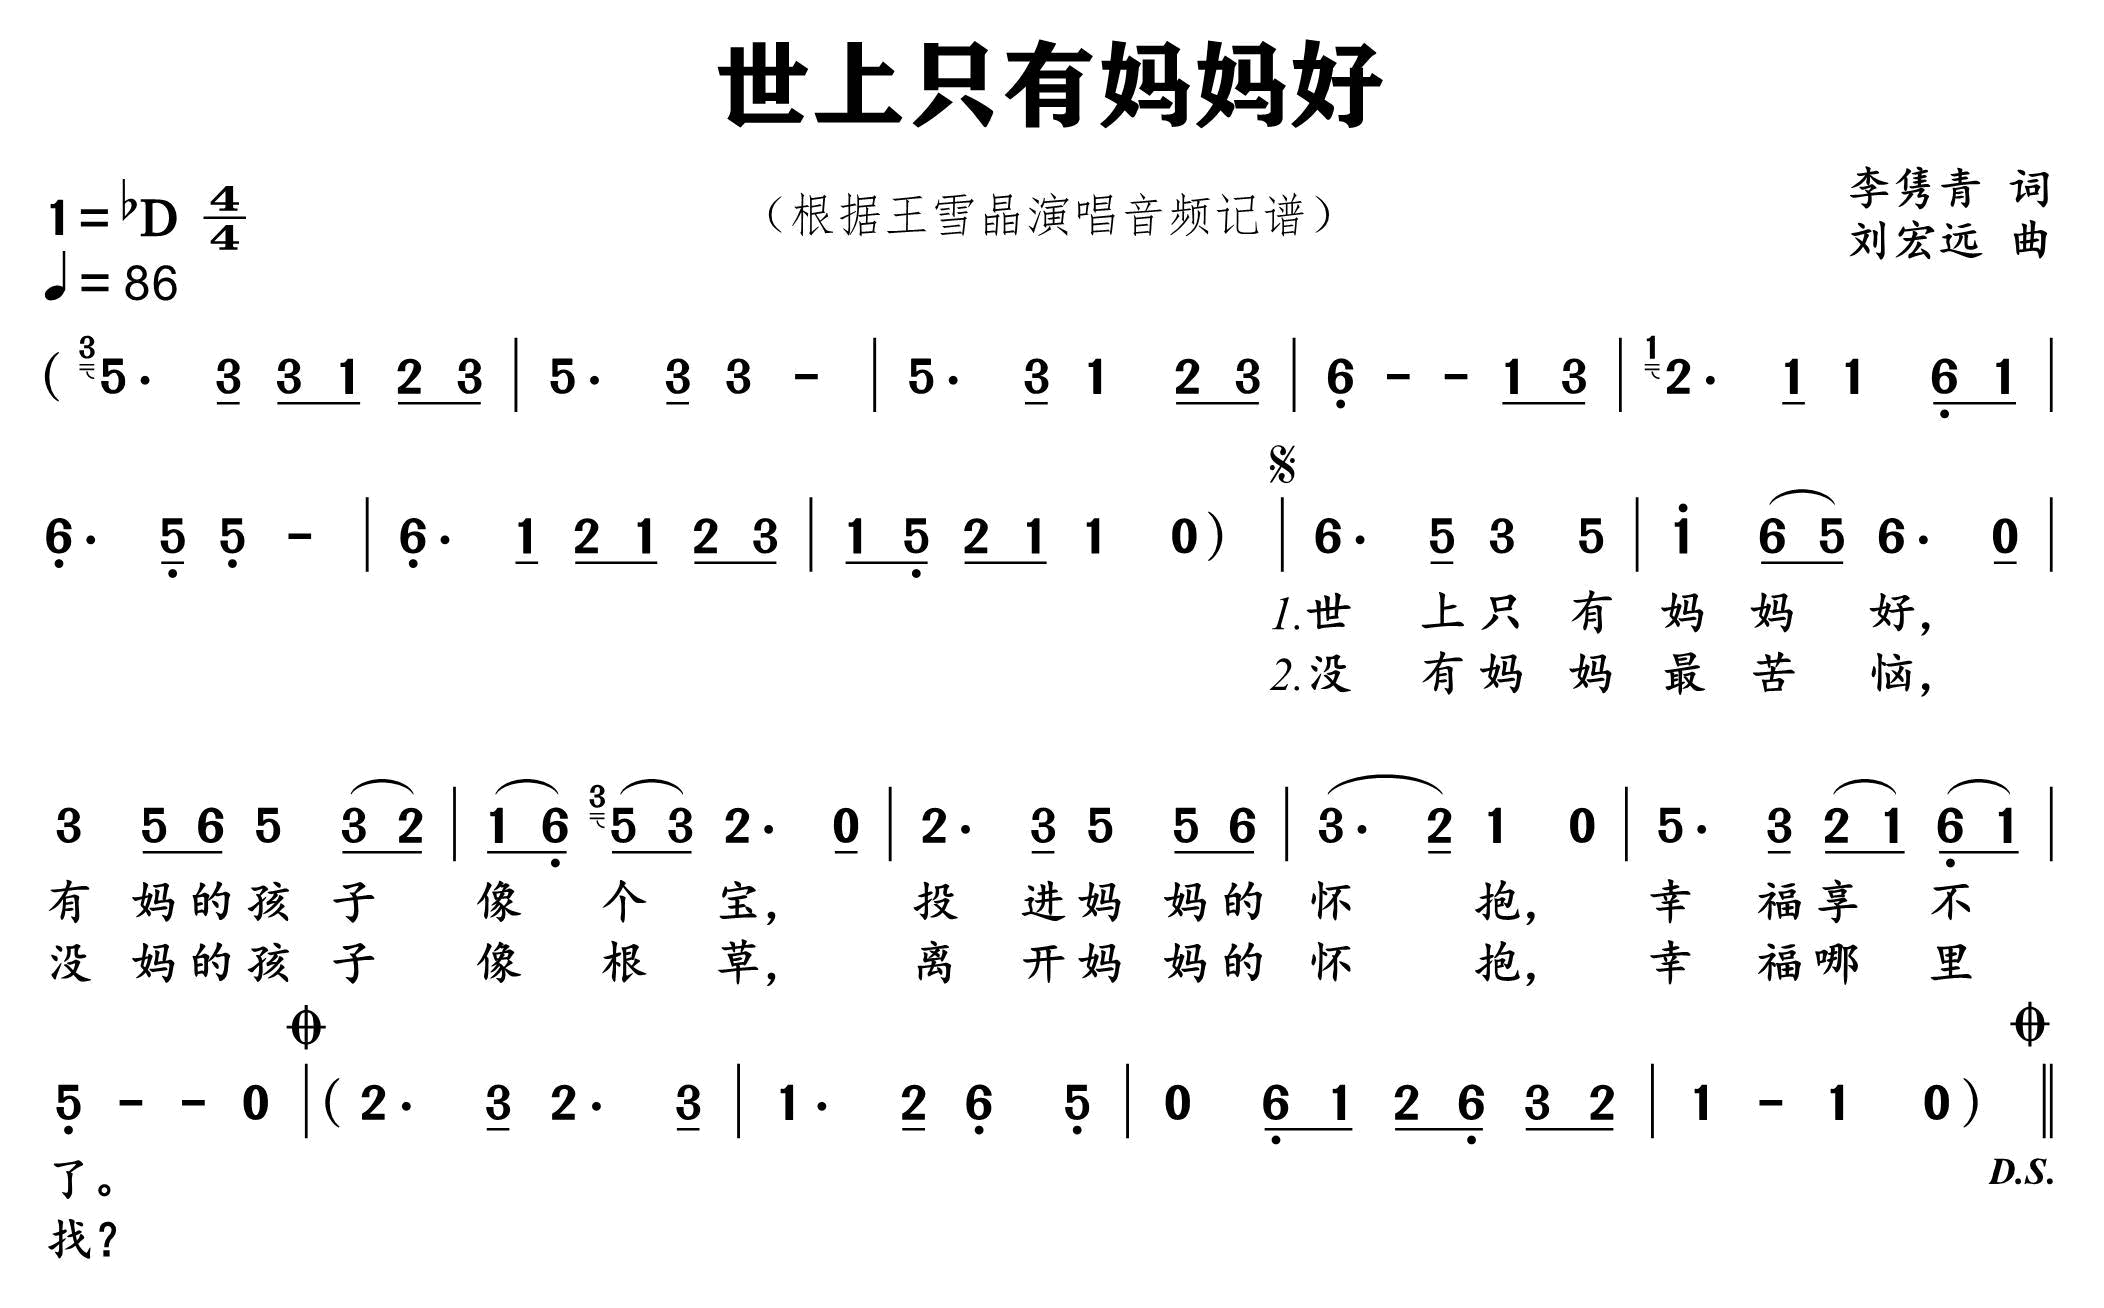
\includegraphics[width=\textwidth]{dongxiao/IMG_0854-世上只有妈妈好.png}
\section{鐘聲}                  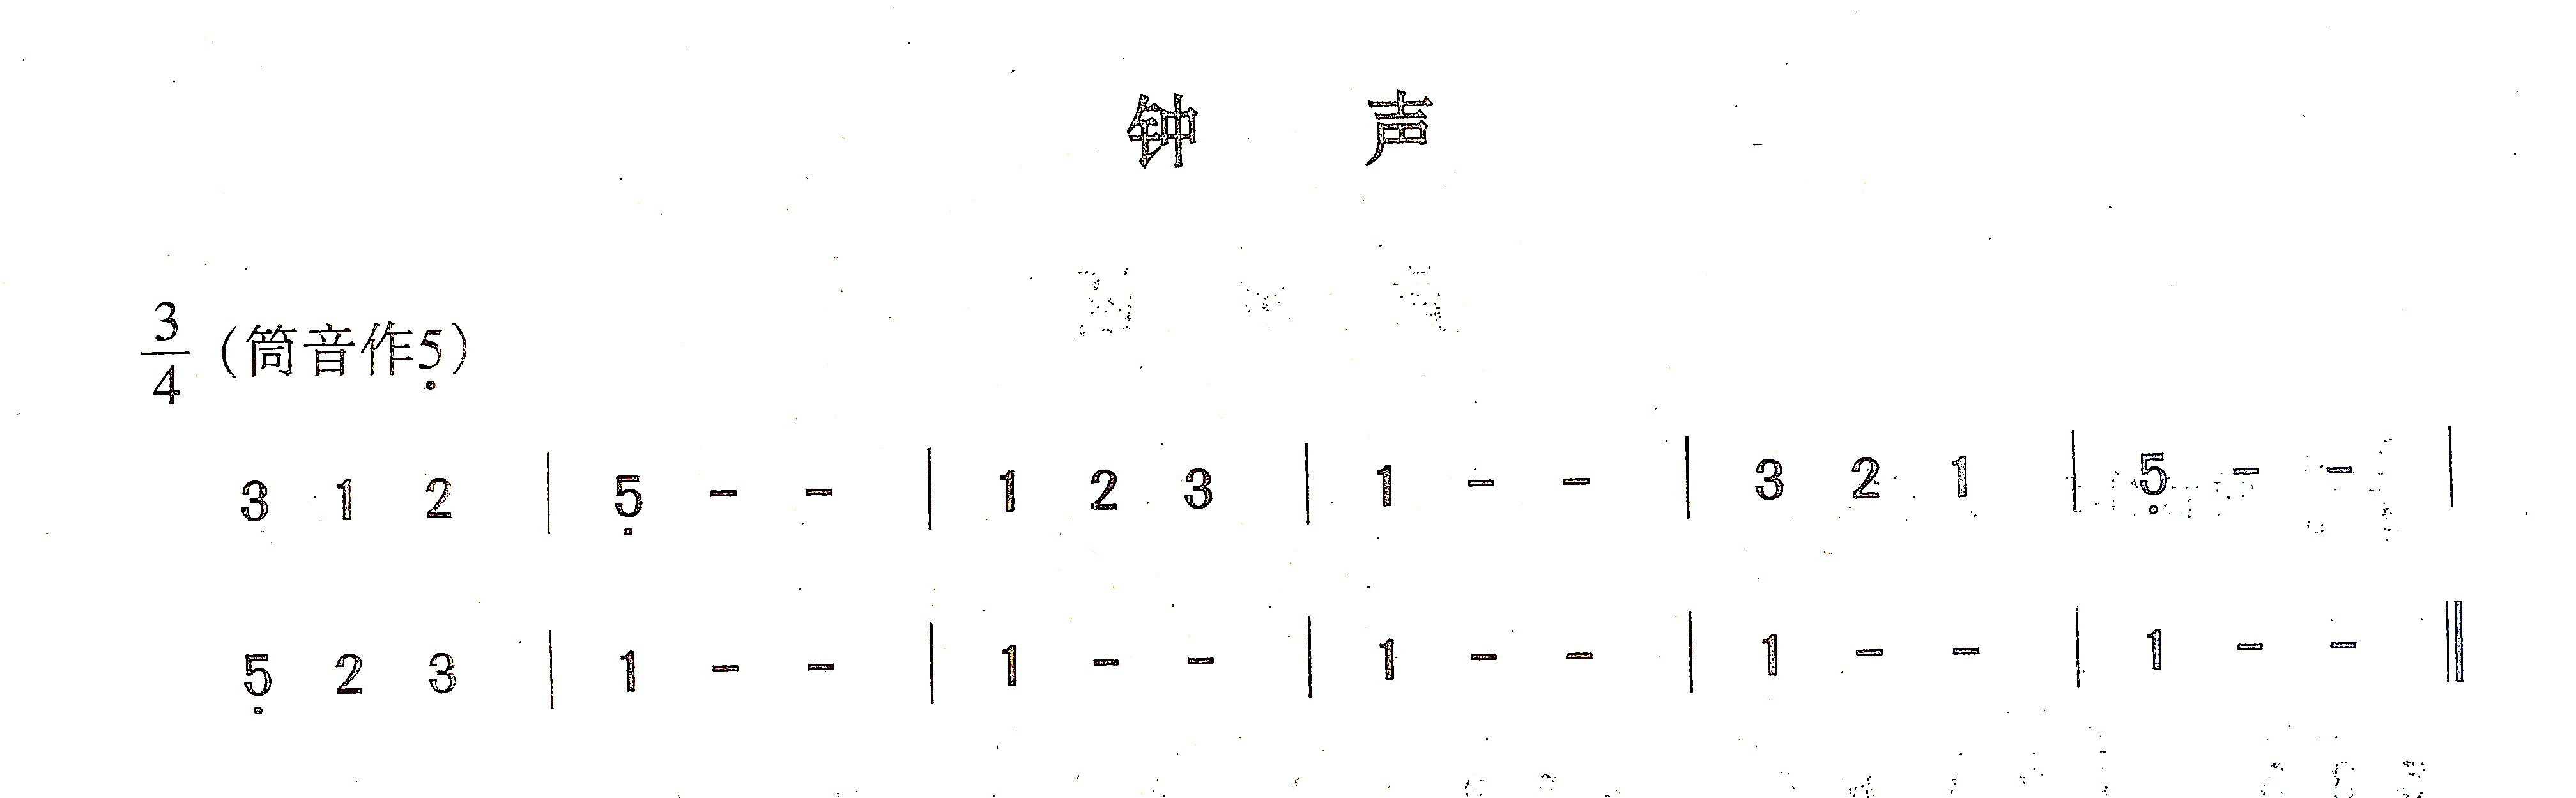
\includegraphics[width=\textwidth]{dongxiao/20200711-钟声.jpg}
\section{小草}                  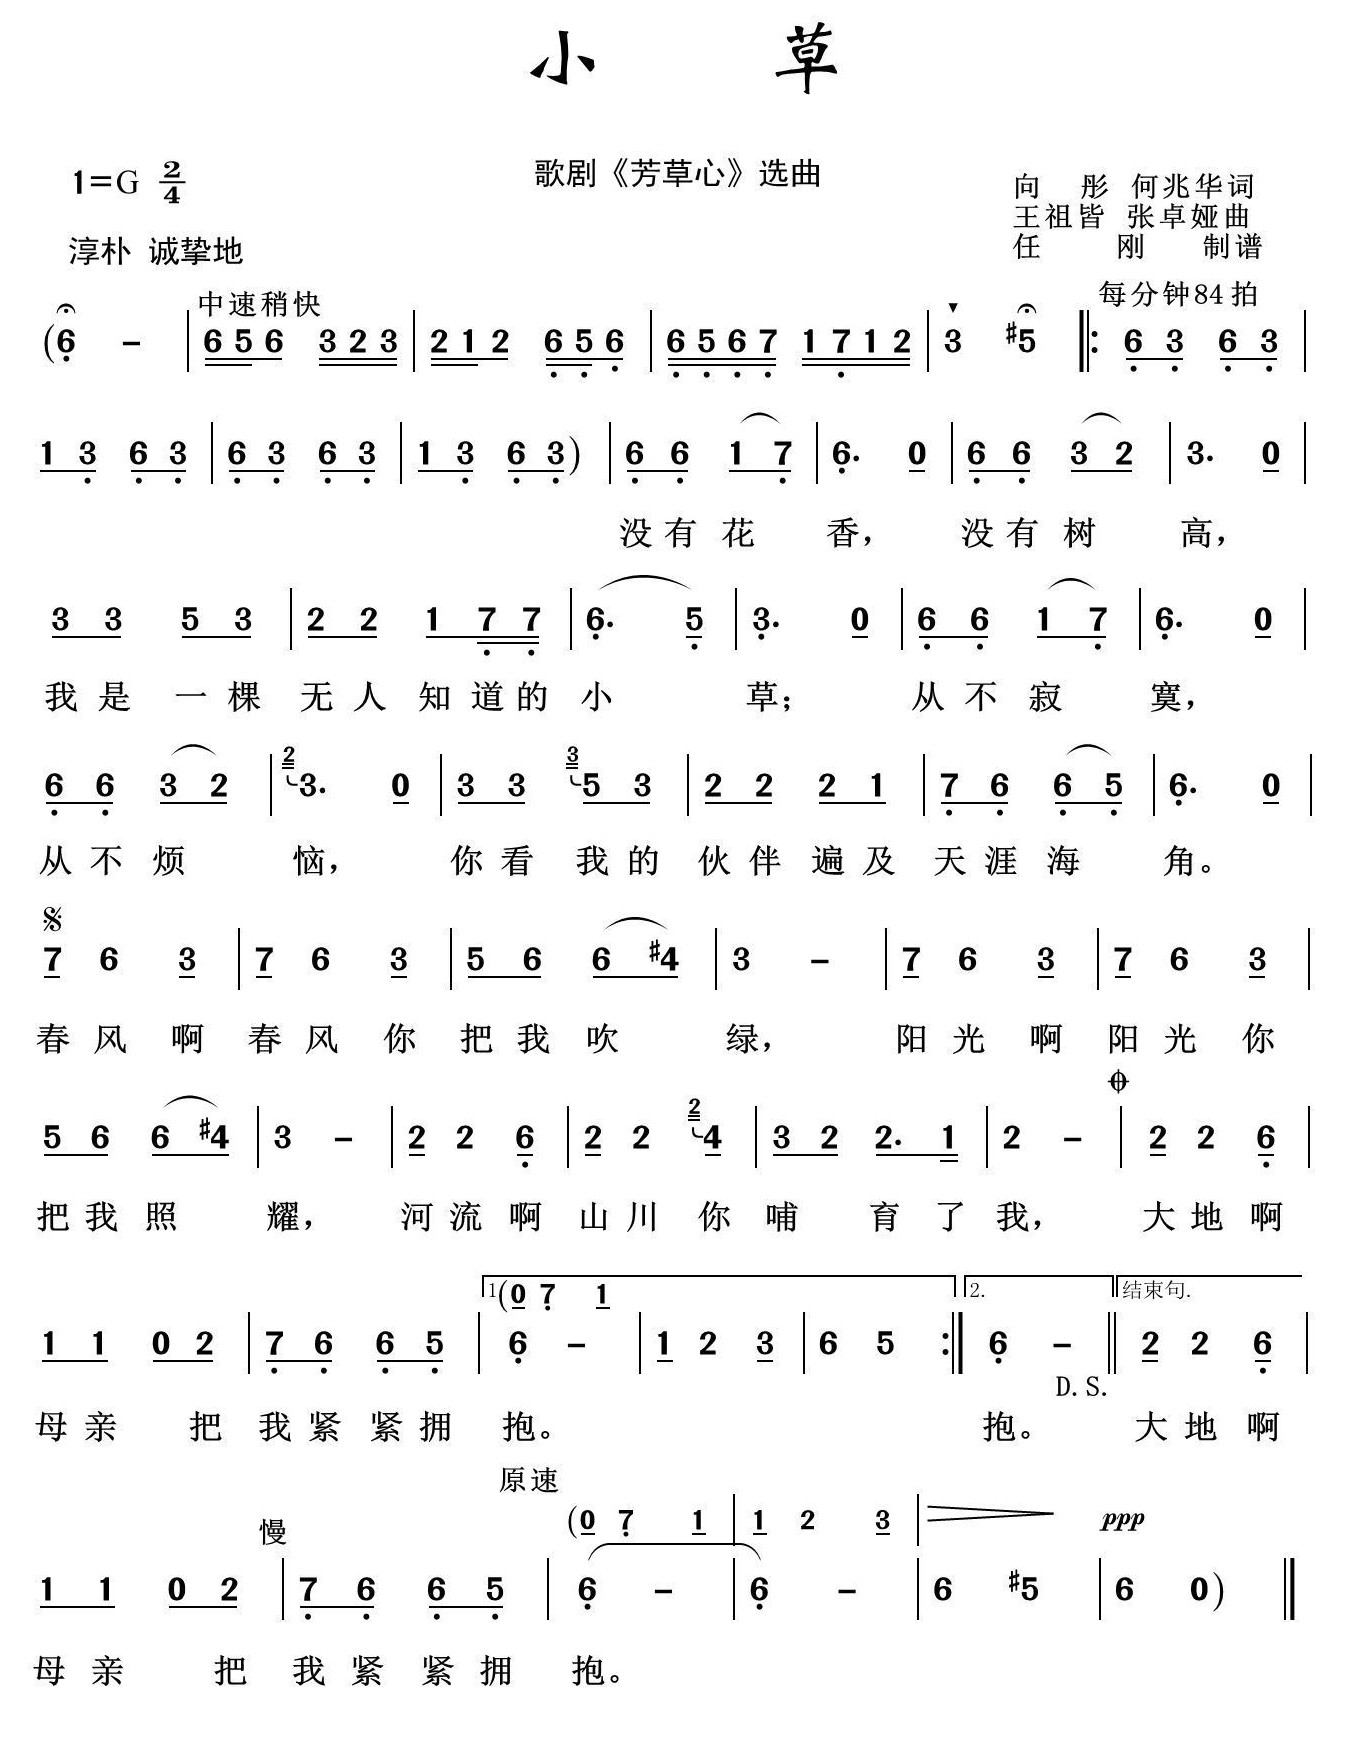
\includegraphics[width=\textwidth]{rpi400/20210131小草.jpeg}
\section{寒山僧踪}              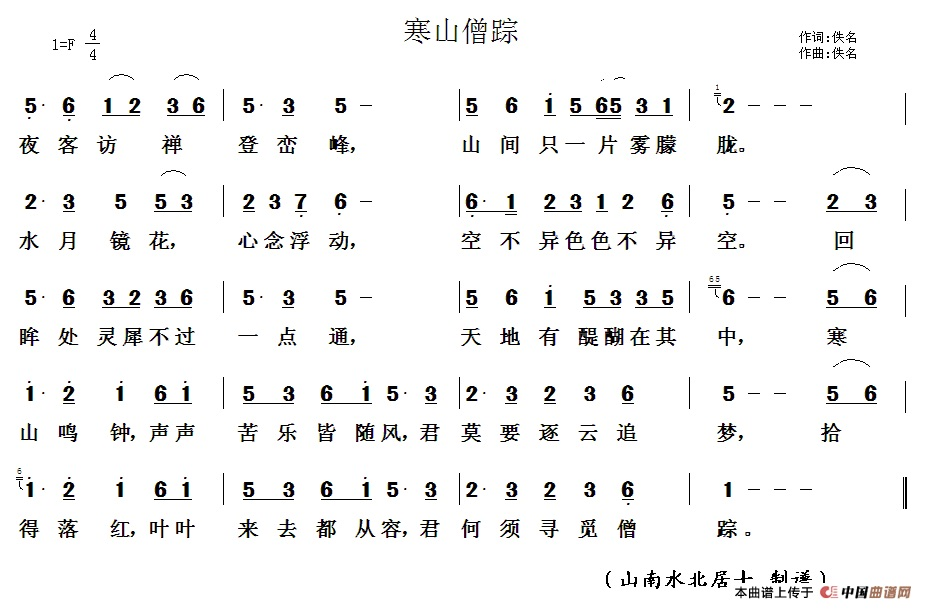
\includegraphics[width=\textwidth]{dongxiao/20200710-寒山僧踪.jpg}
\section{般若}                  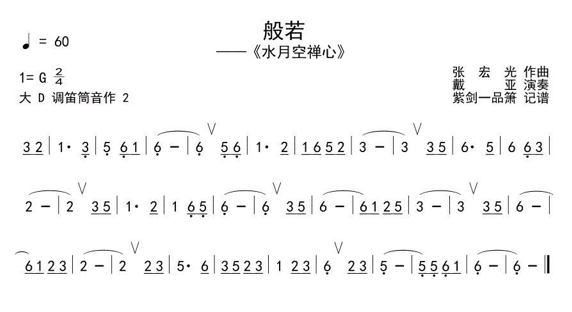
\includegraphics[width=\textwidth]{macos/20210205般若.png}
\section{雪梅疏影}              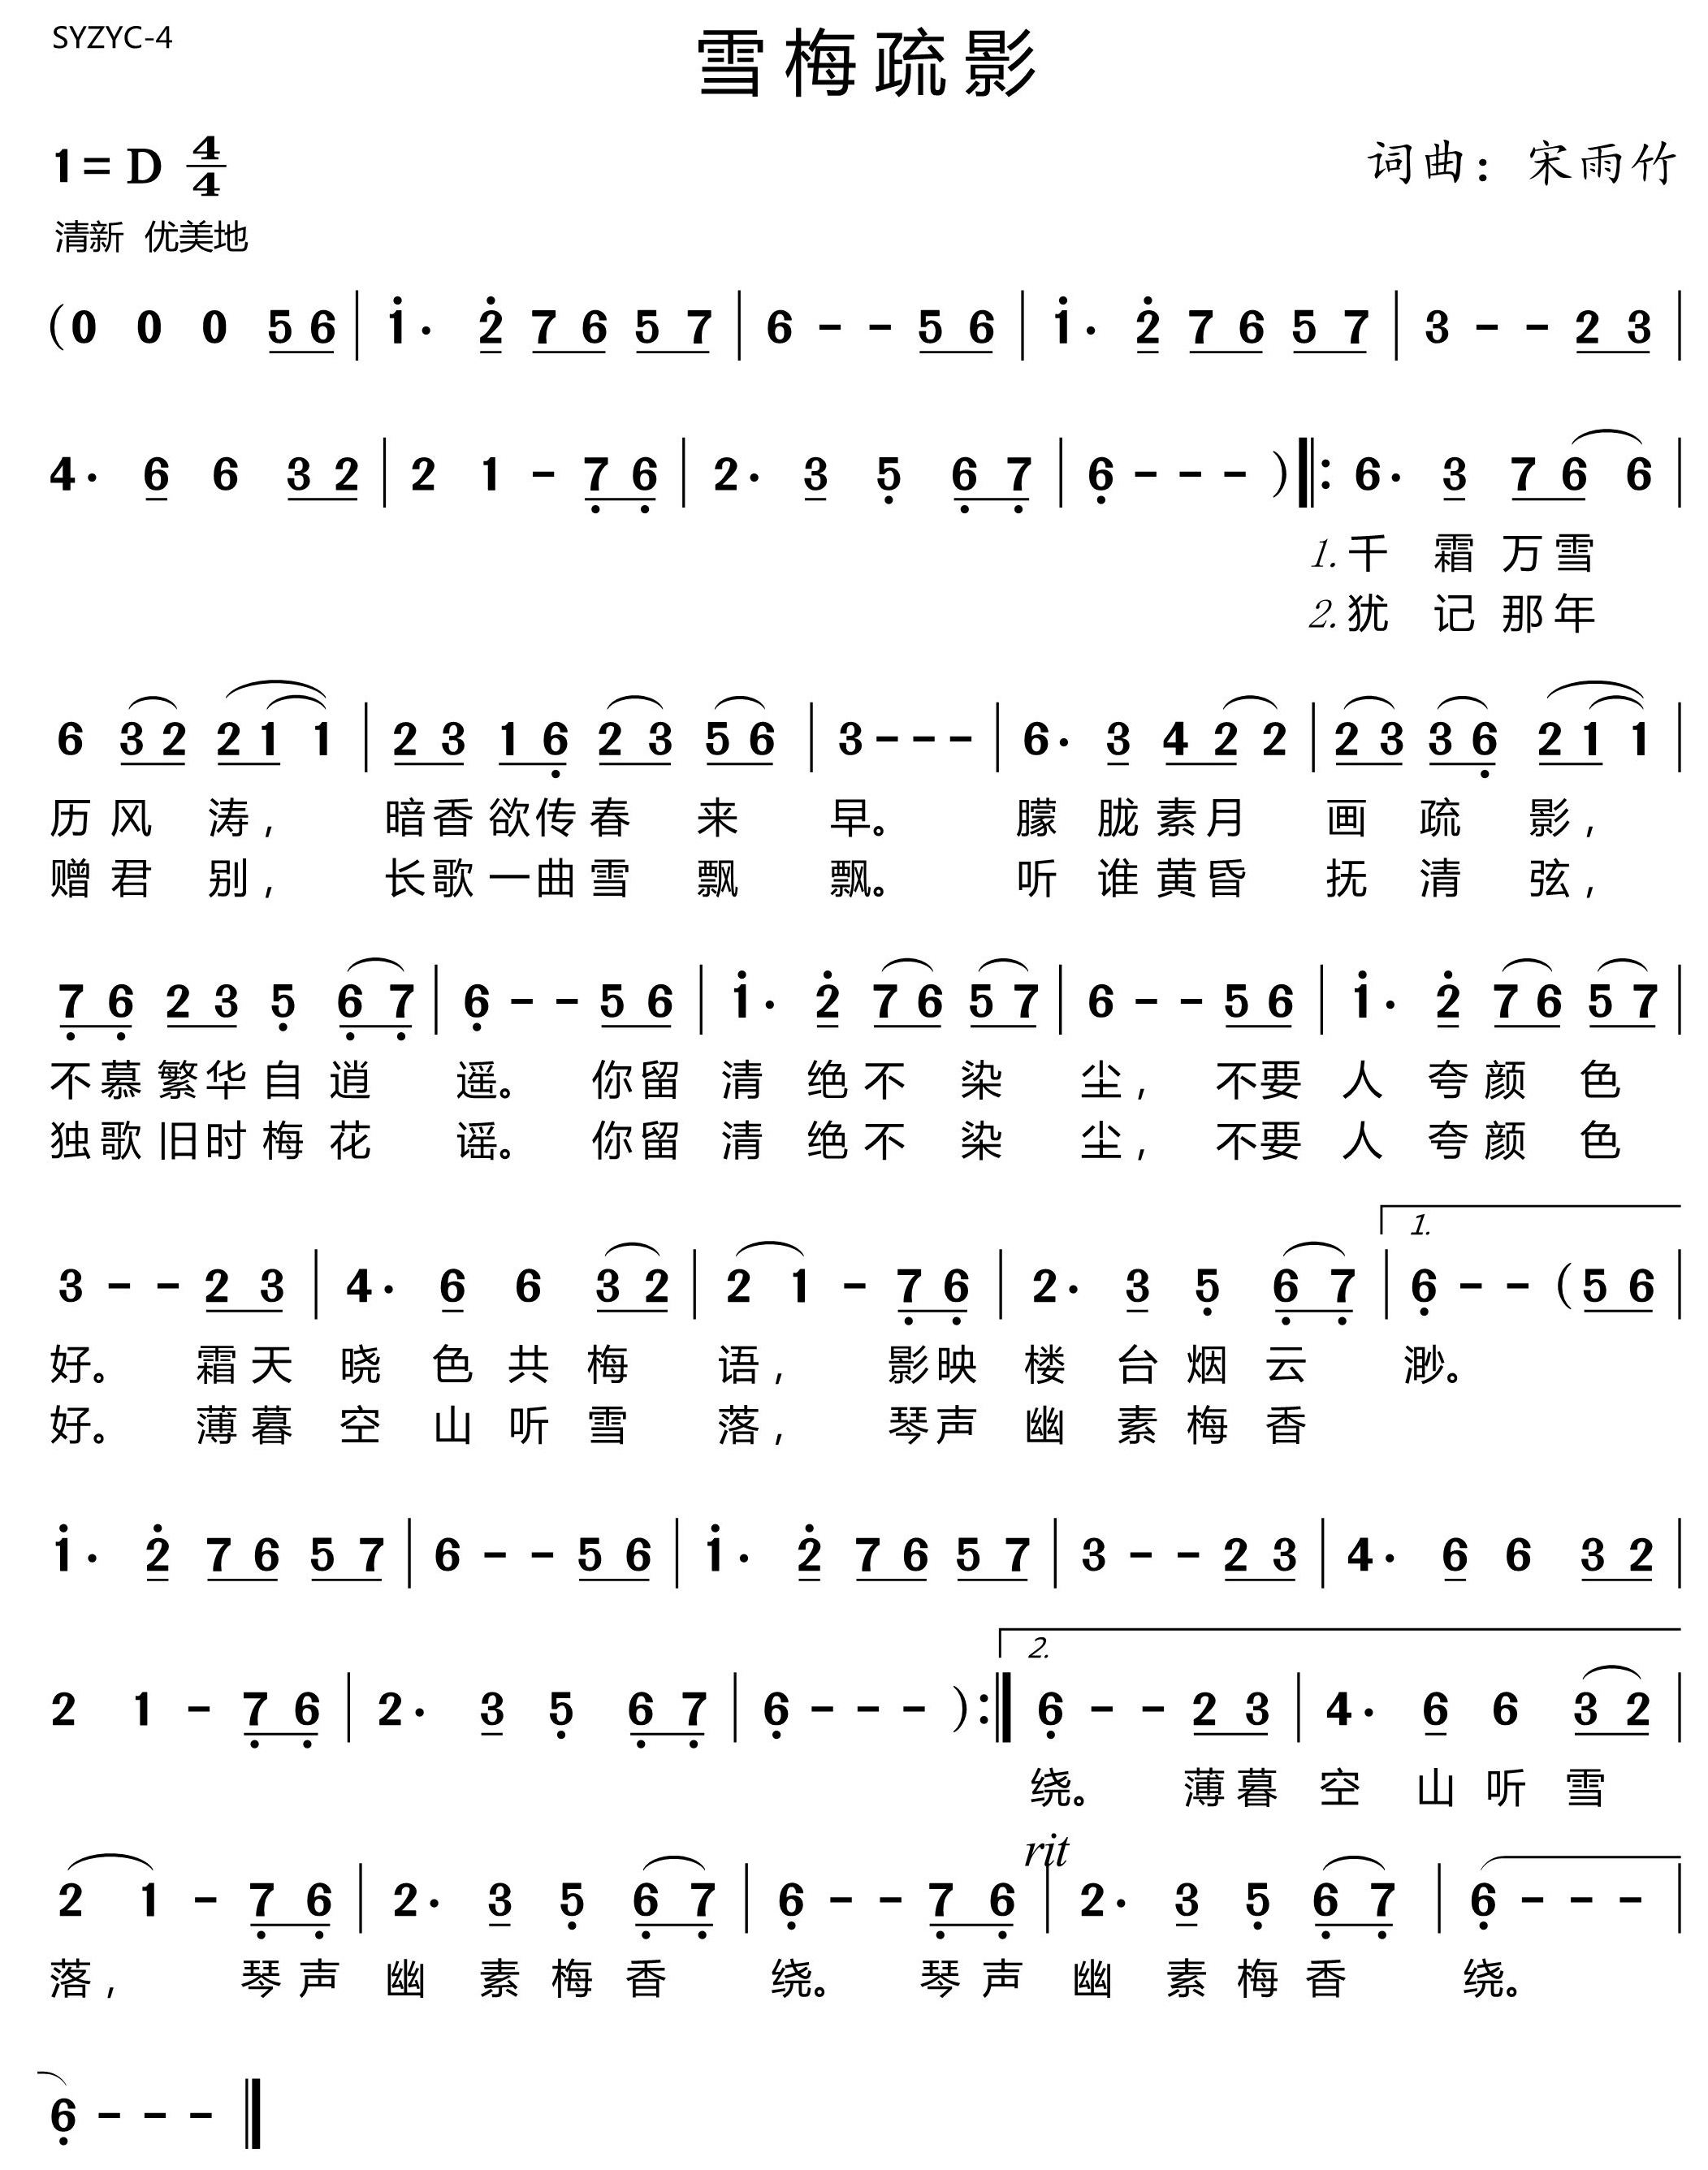
\includegraphics[width=0.9\textwidth]{dongxiao/20200725-雪梅疏影}
\section{静夜思}                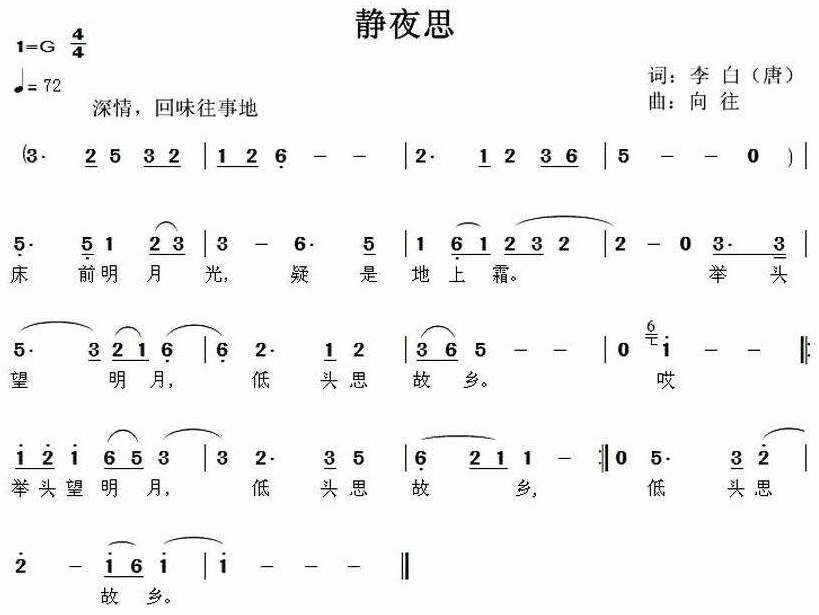
\includegraphics[width=0.9\textwidth]{dongxiao/20200411-静夜思}
\section{饮酒}                  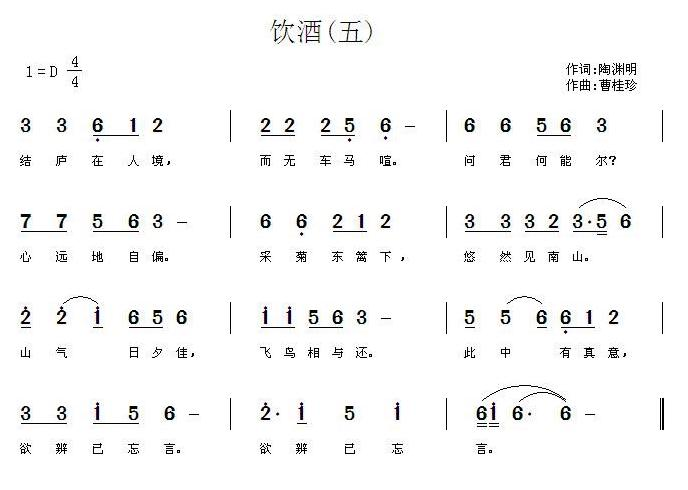
\includegraphics[width=\textwidth]{dongxiao/20200808-饮酒-陶渊明.jpg}
\section{长安忆}                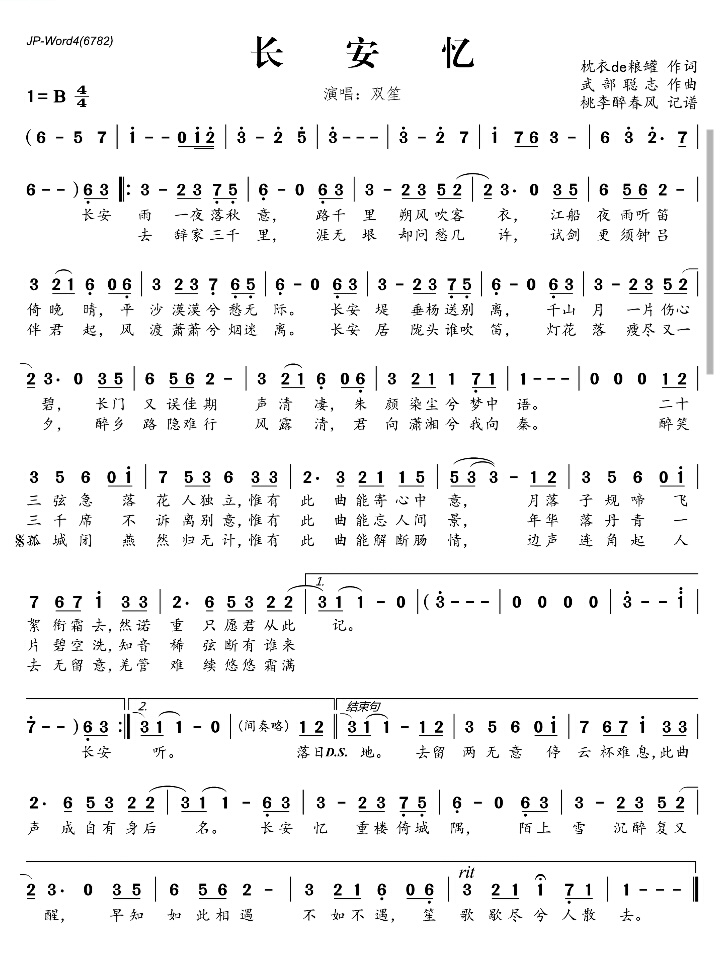
\includegraphics[width=0.95\textwidth]{rpi400/20210123-长安忆.jpg}
\section{橄榄树} 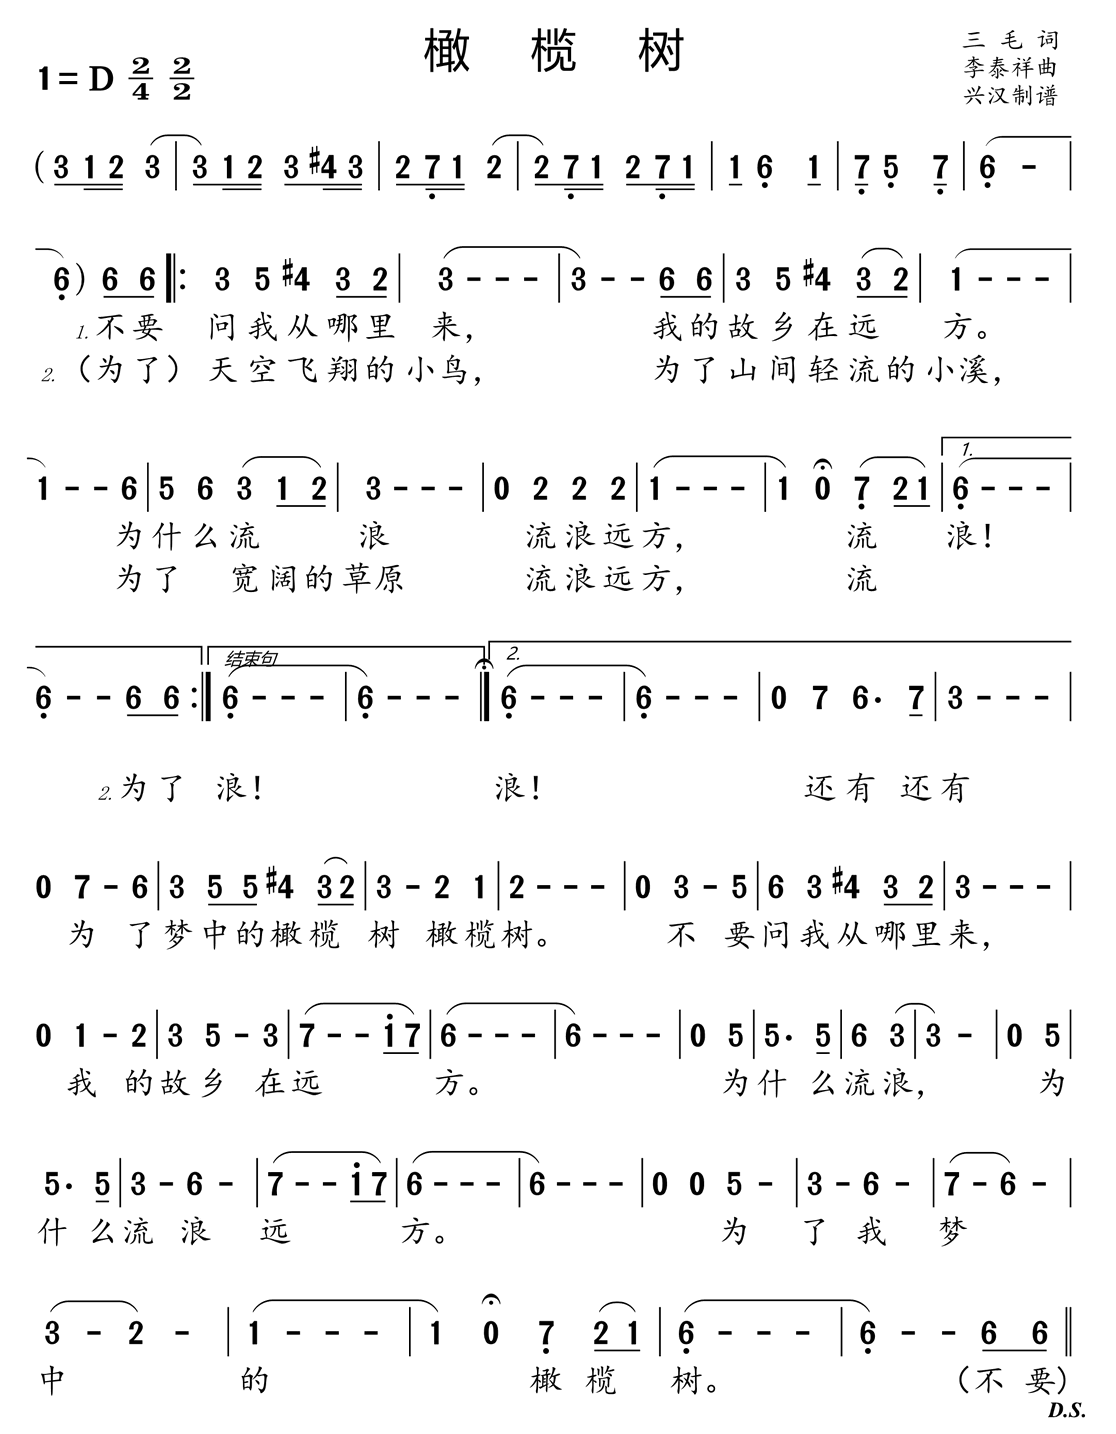
\includegraphics[width=\textwidth]{rpi400/20210206橄榄树.png}
\section{姜子牙主题曲} 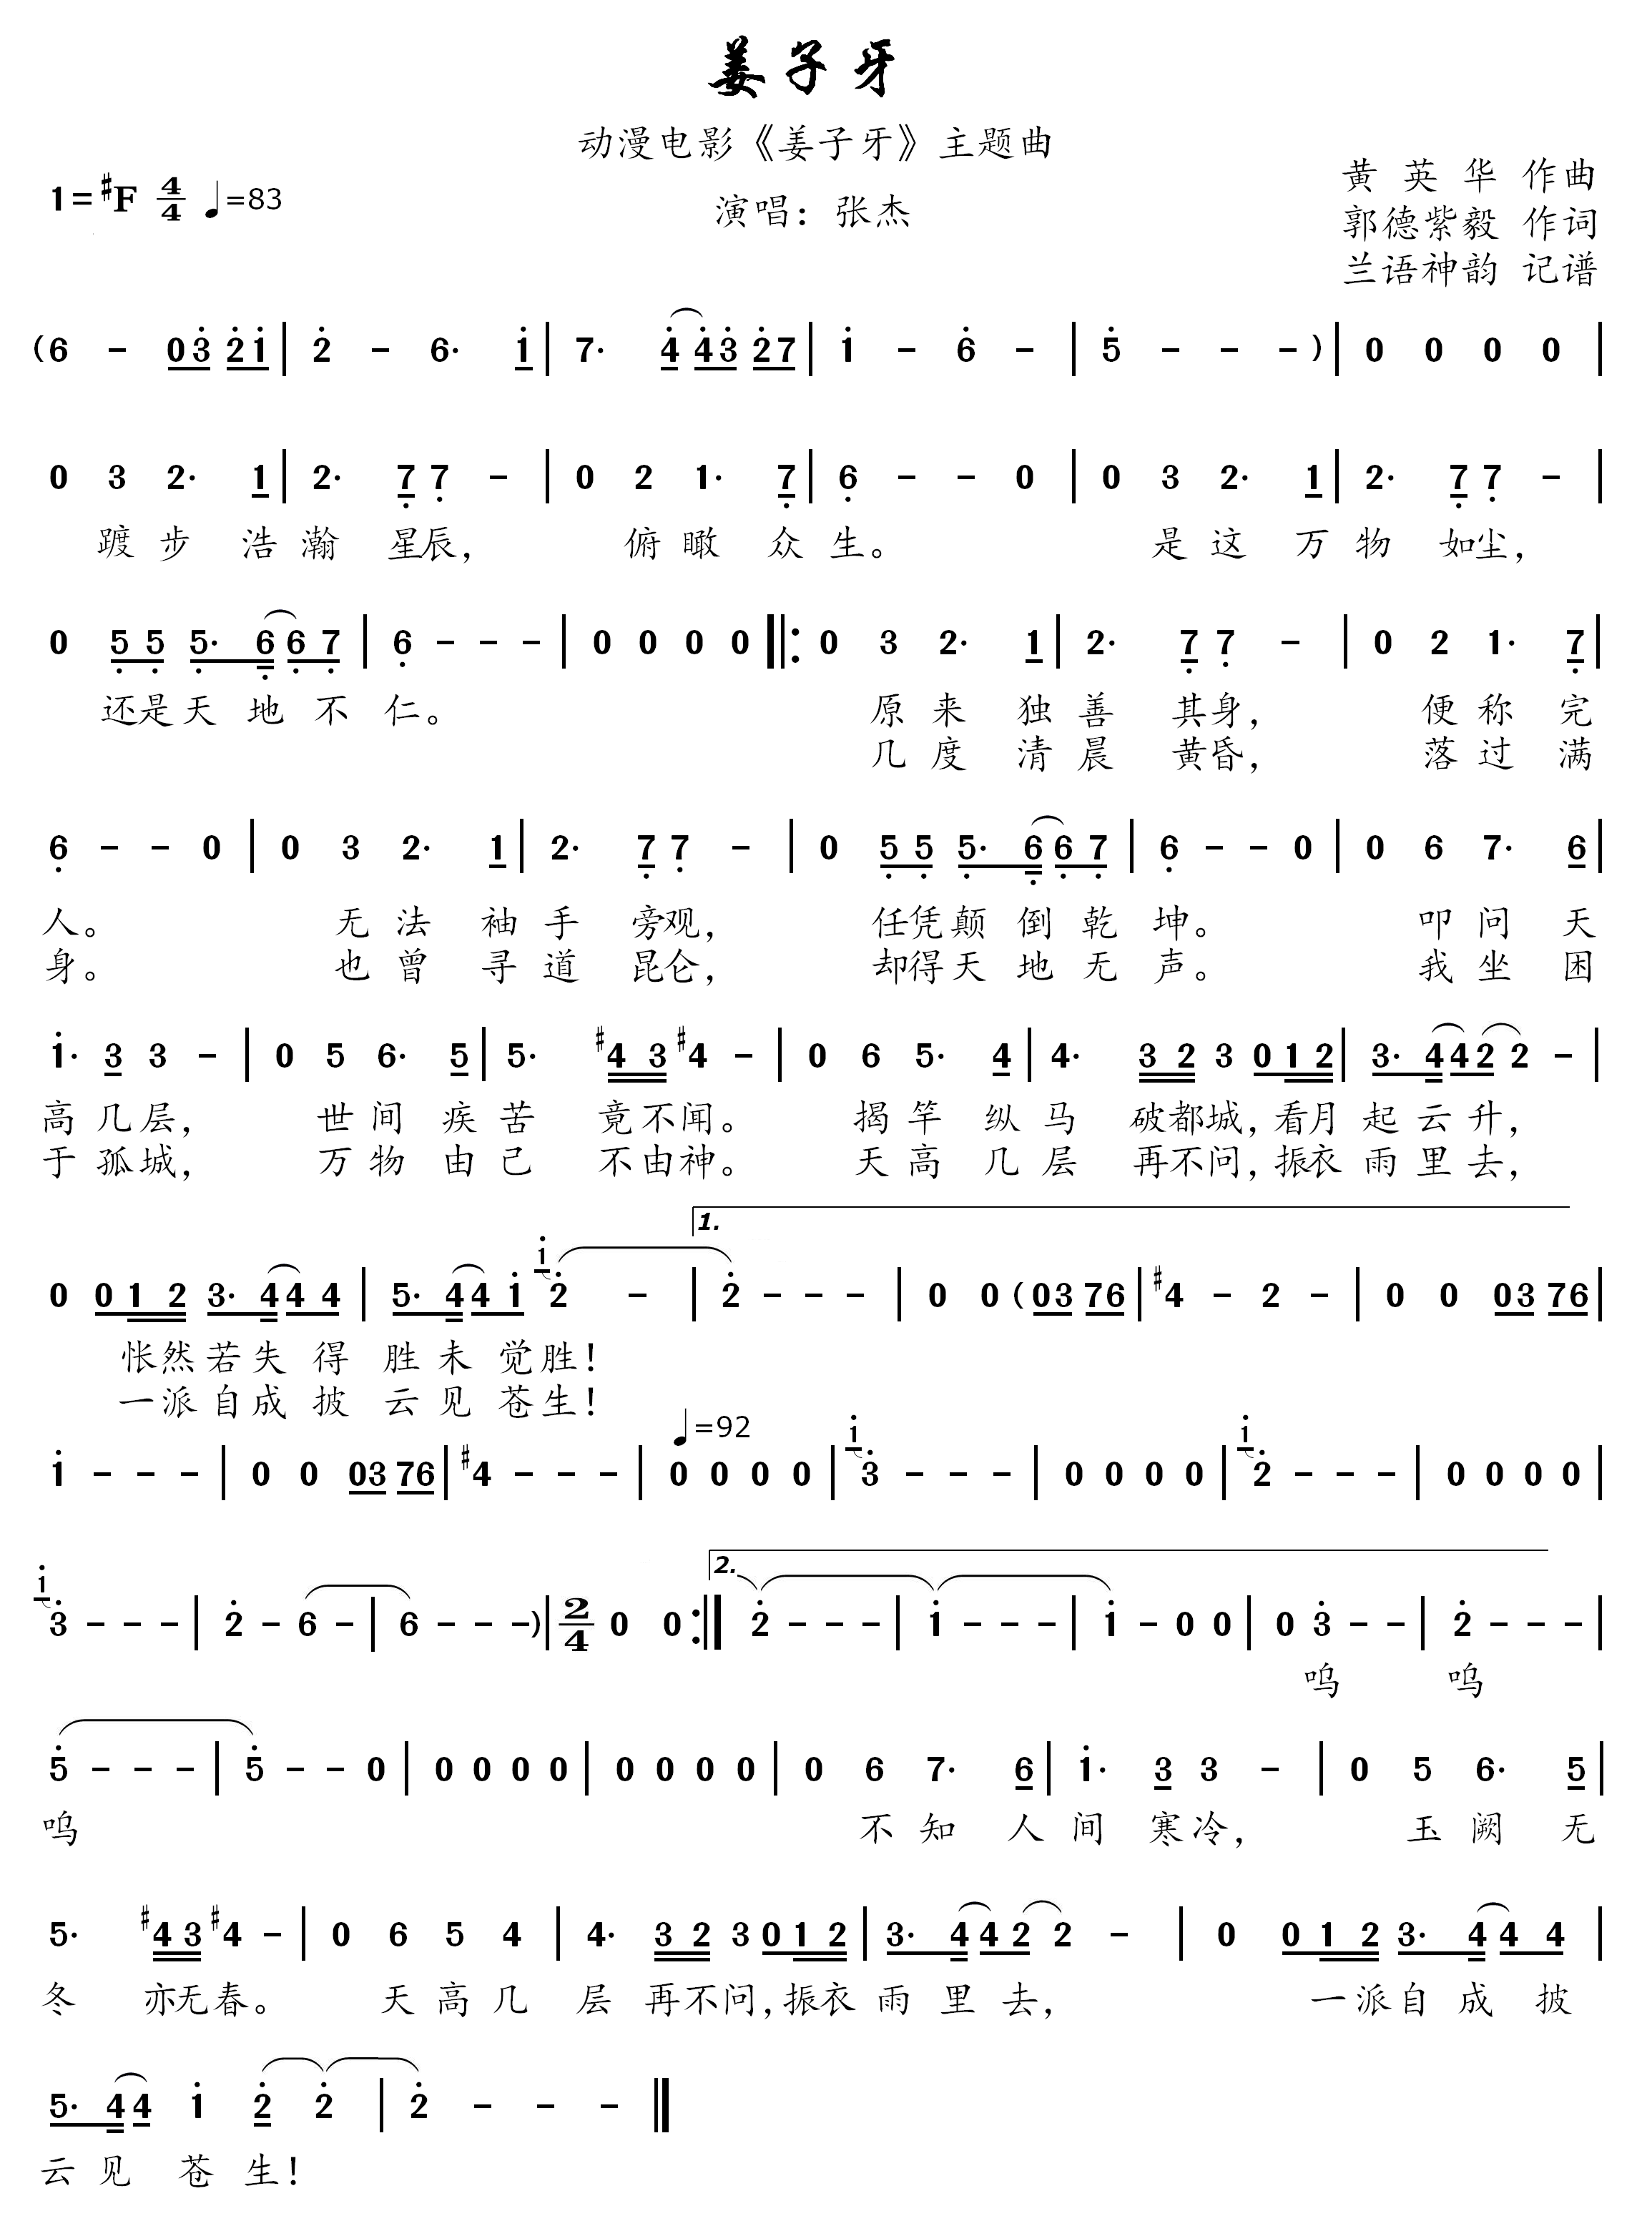
\includegraphics[width=\textwidth]{rpi400/20210206姜子牙主题曲.png}
\section{请笃信一个梦} 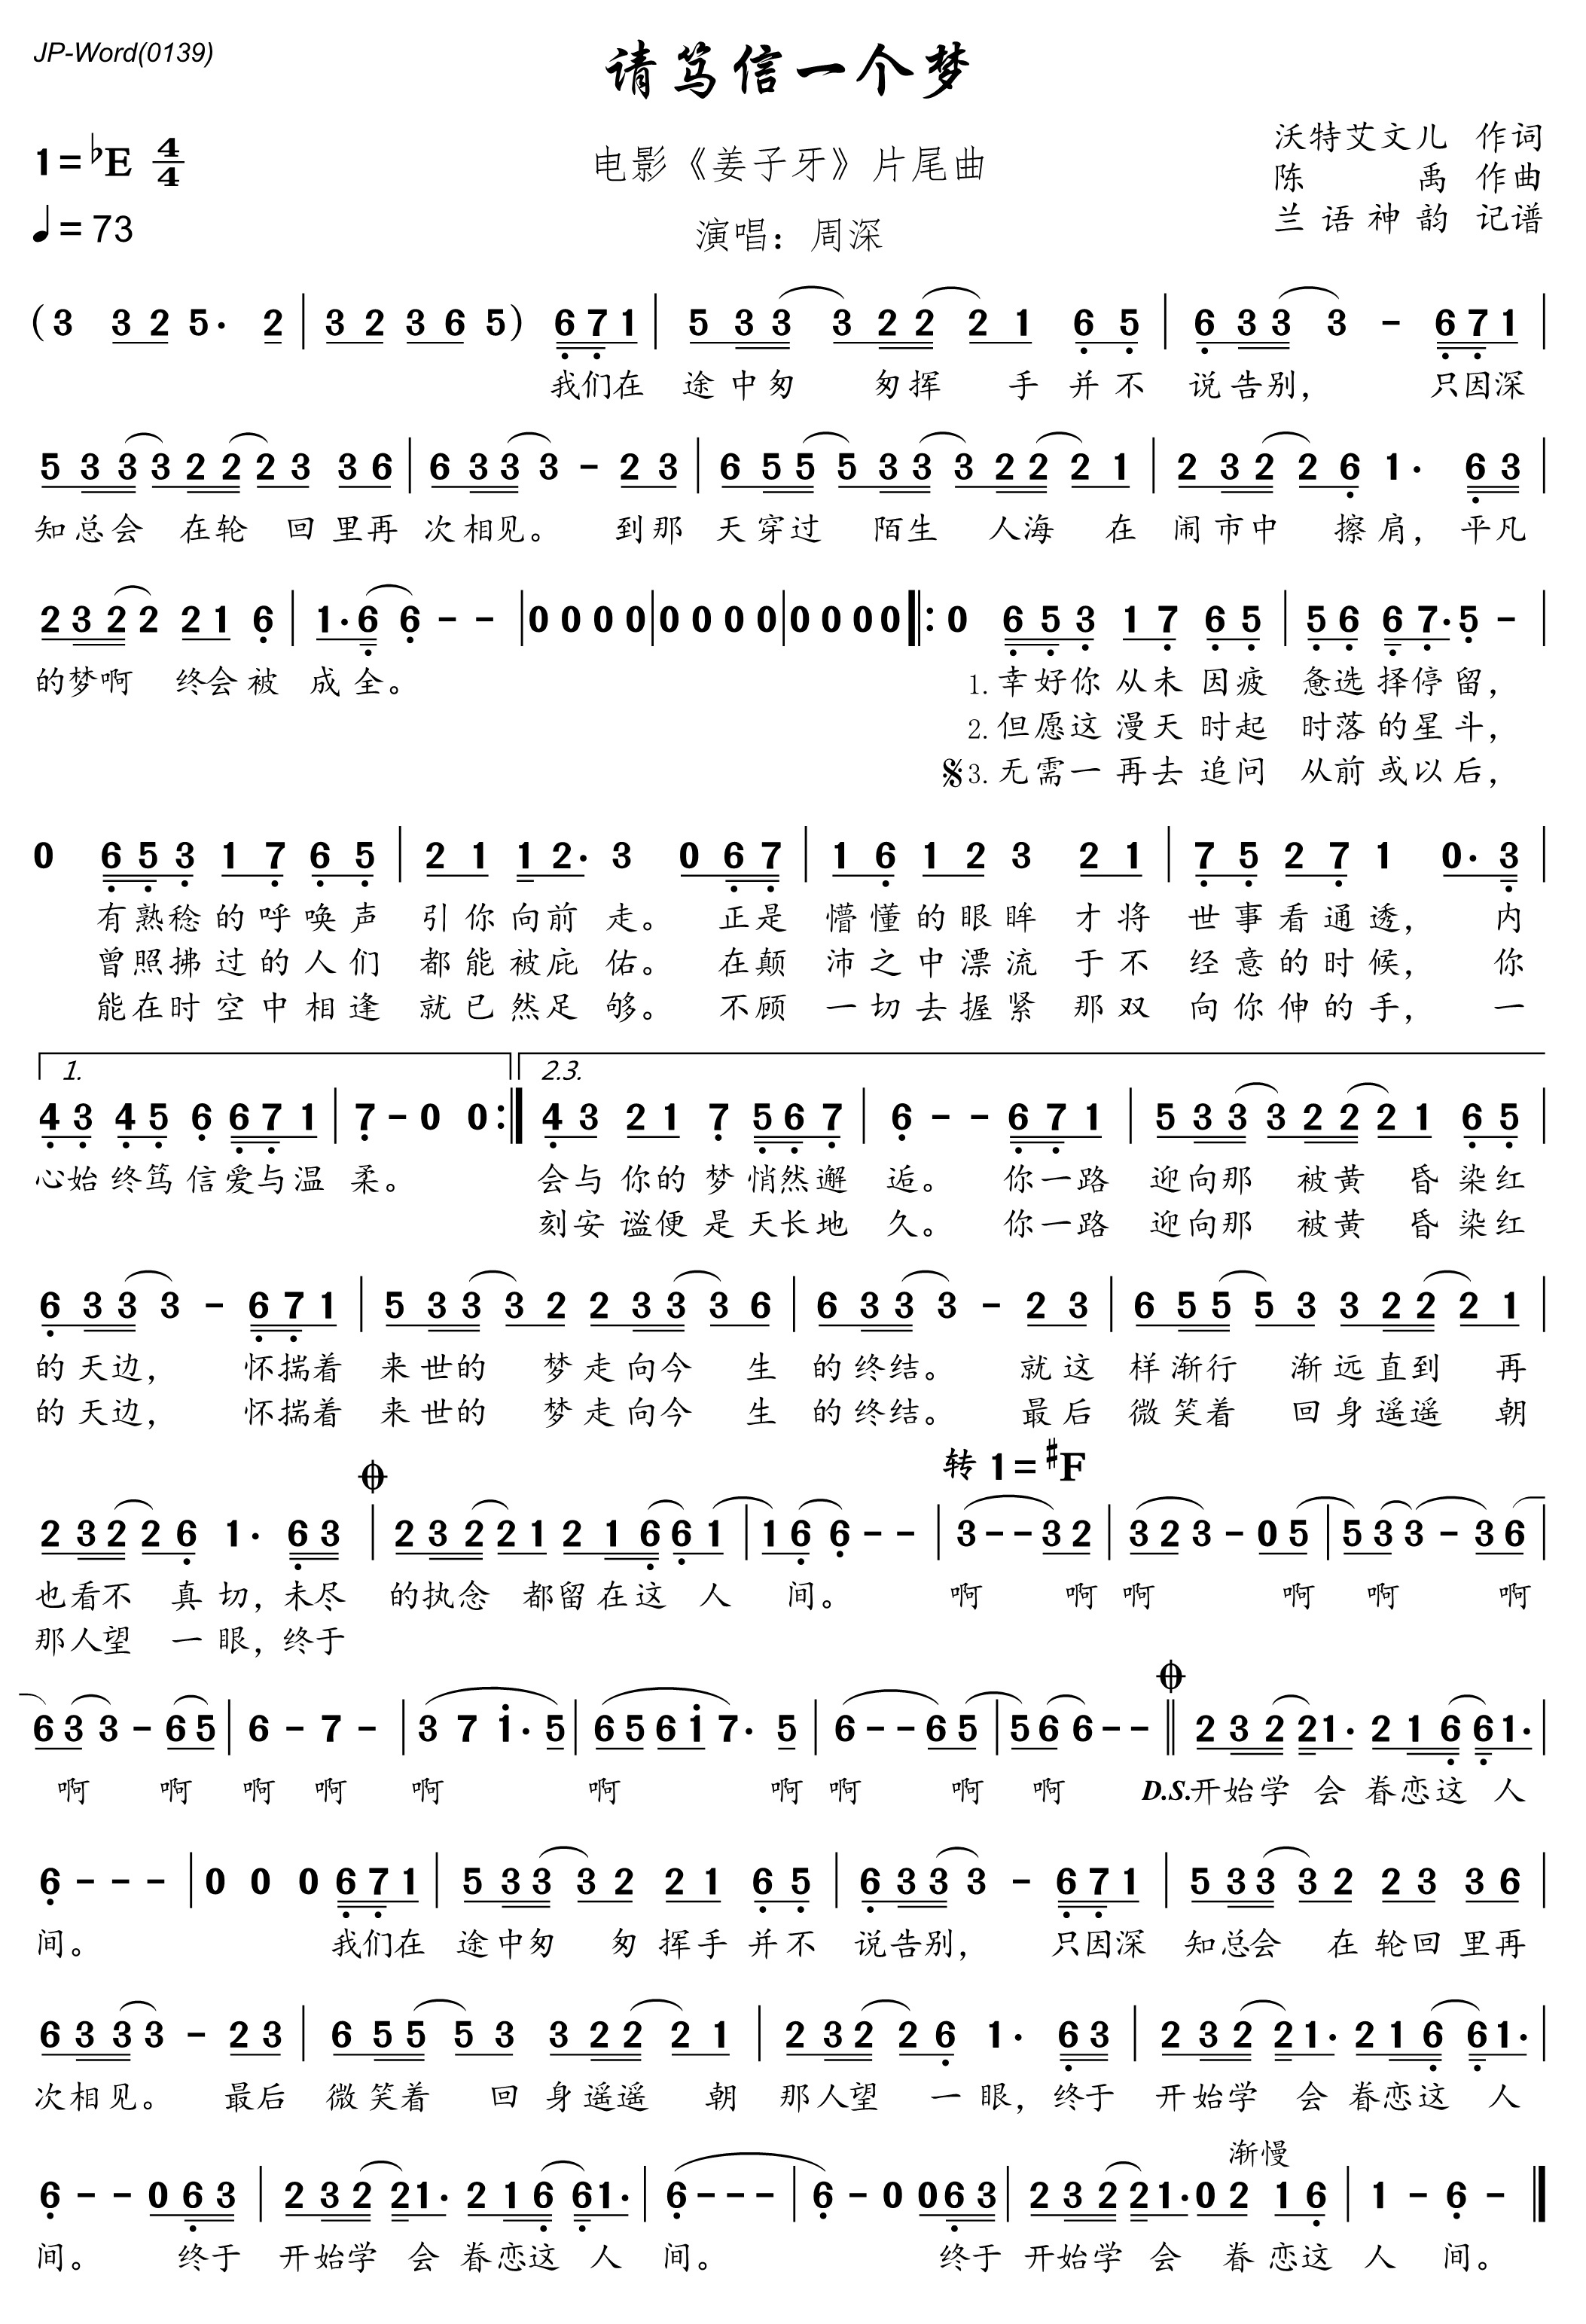
\includegraphics[width=0.85\textwidth]{rpi400/20210206请笃信一个梦.png}
\section{任花落} 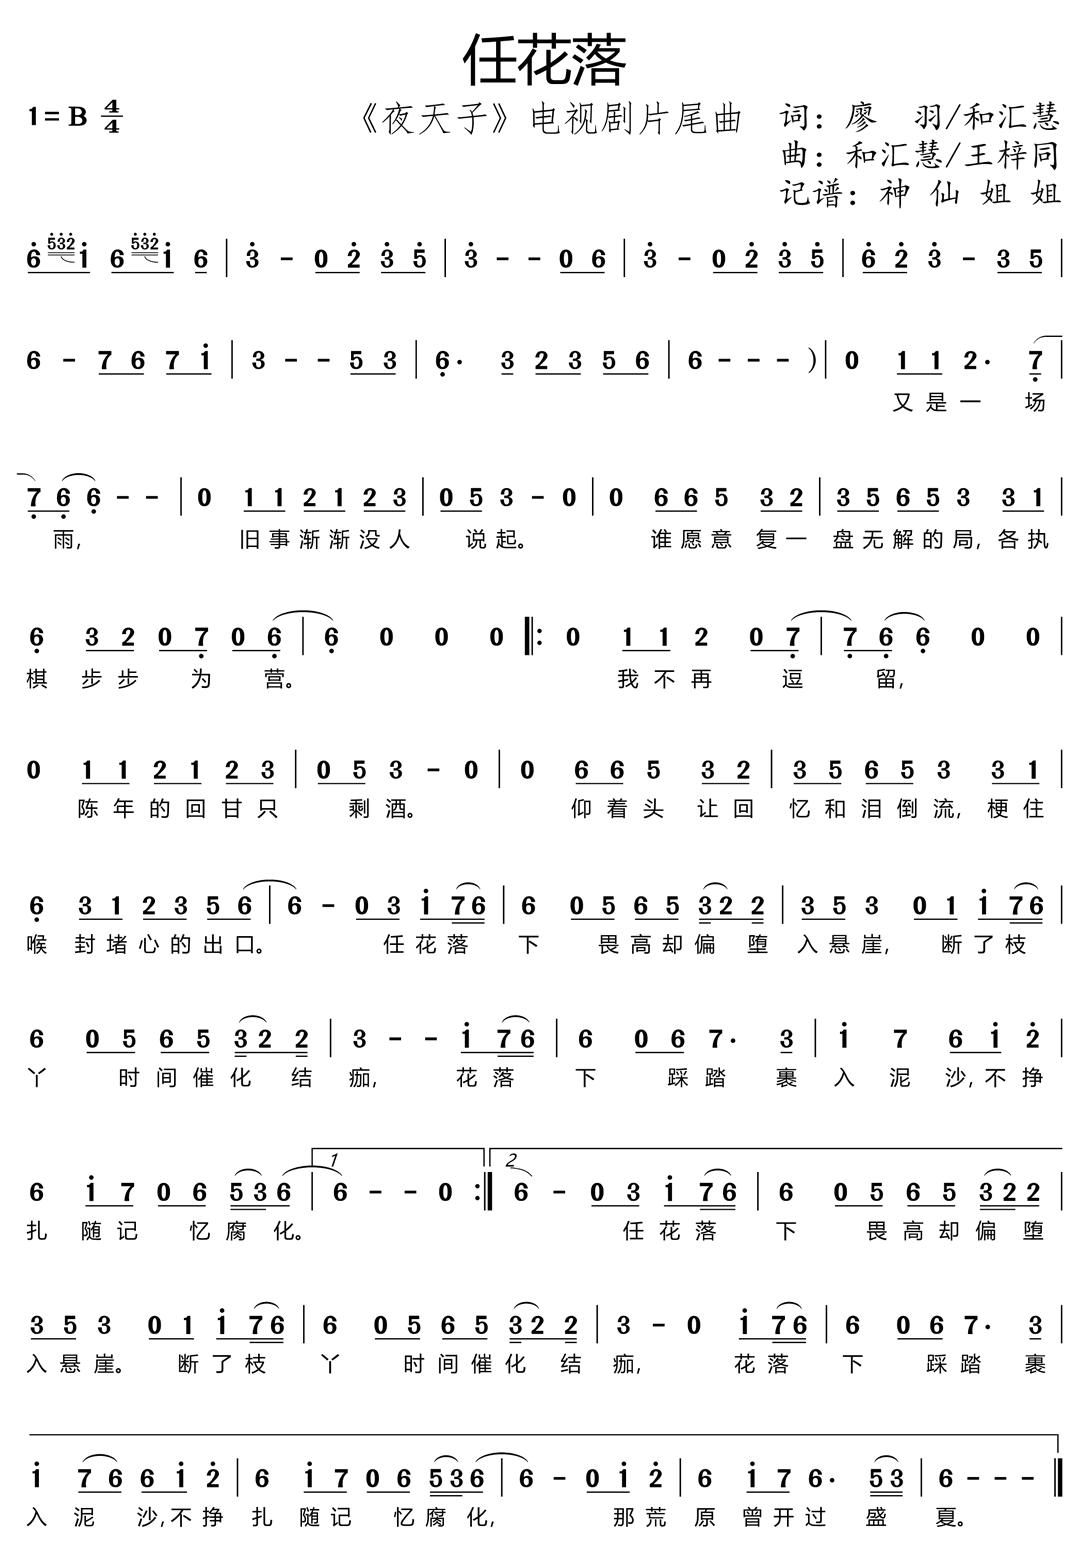
\includegraphics[width=0.9\textwidth]{rpi400/20210206任花落.png}
\section{你真好} 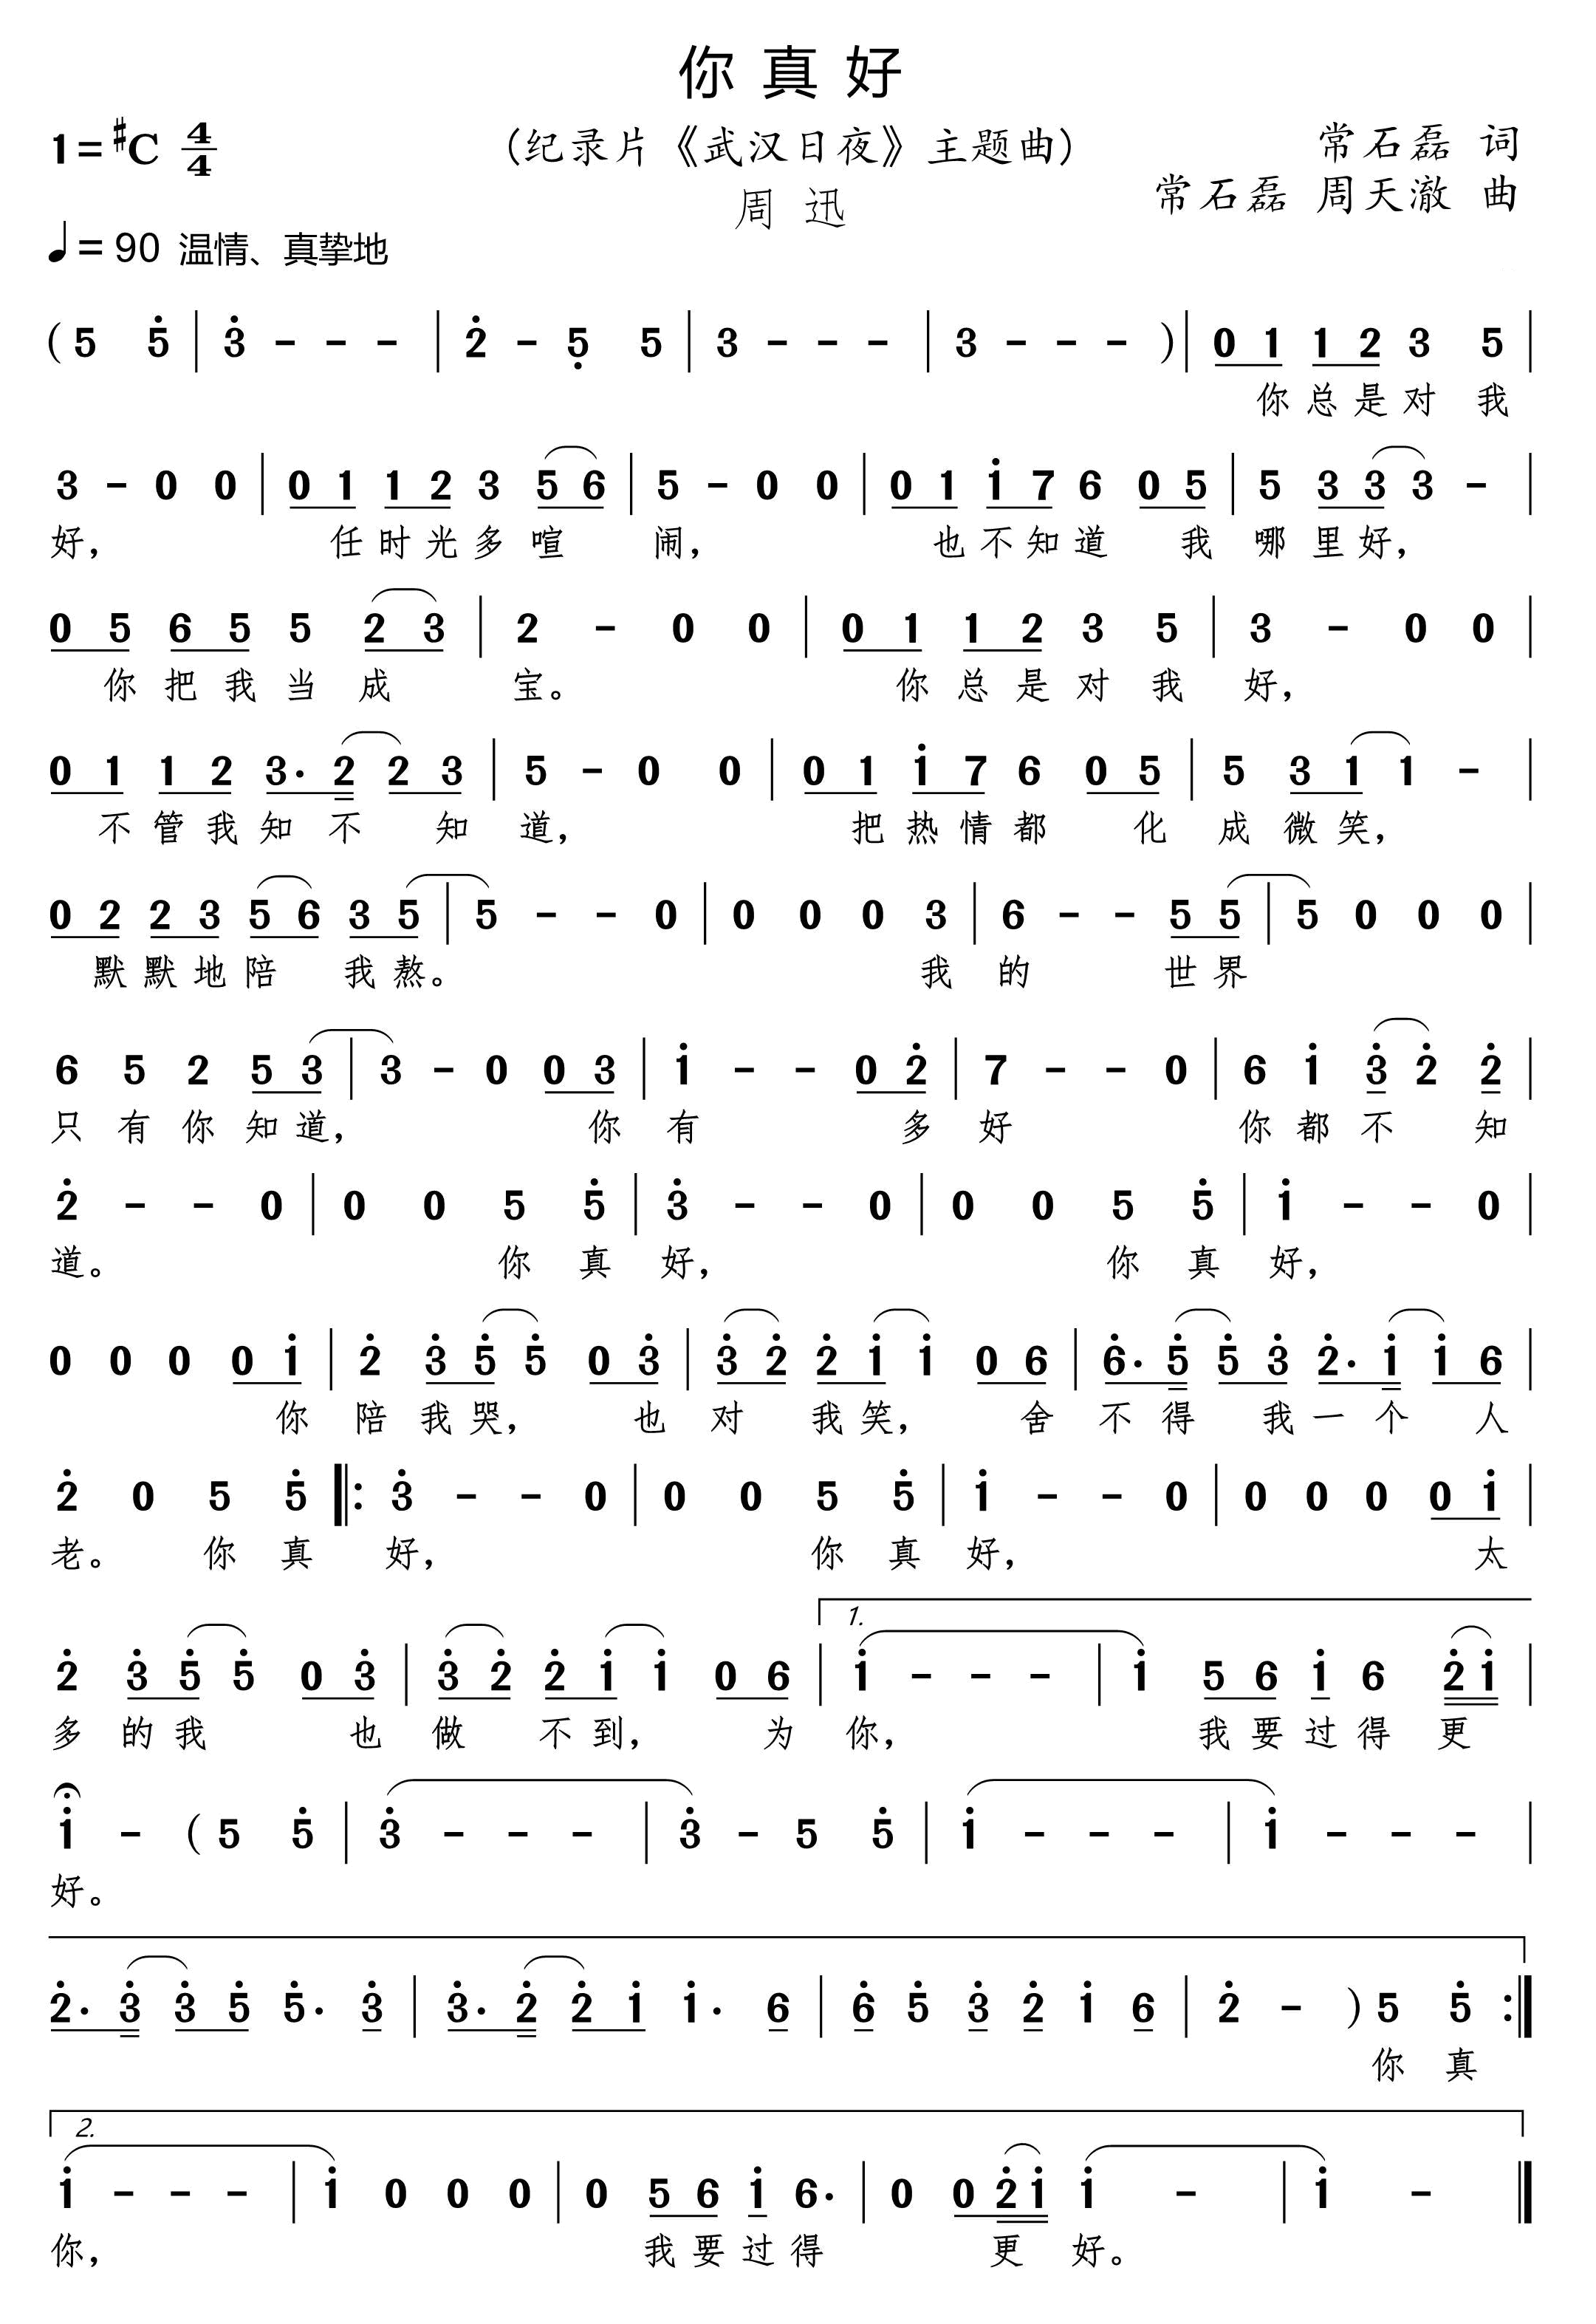
\includegraphics[width=0.9\textwidth]{rpi400/20210206你真好.png}
\section{印记} 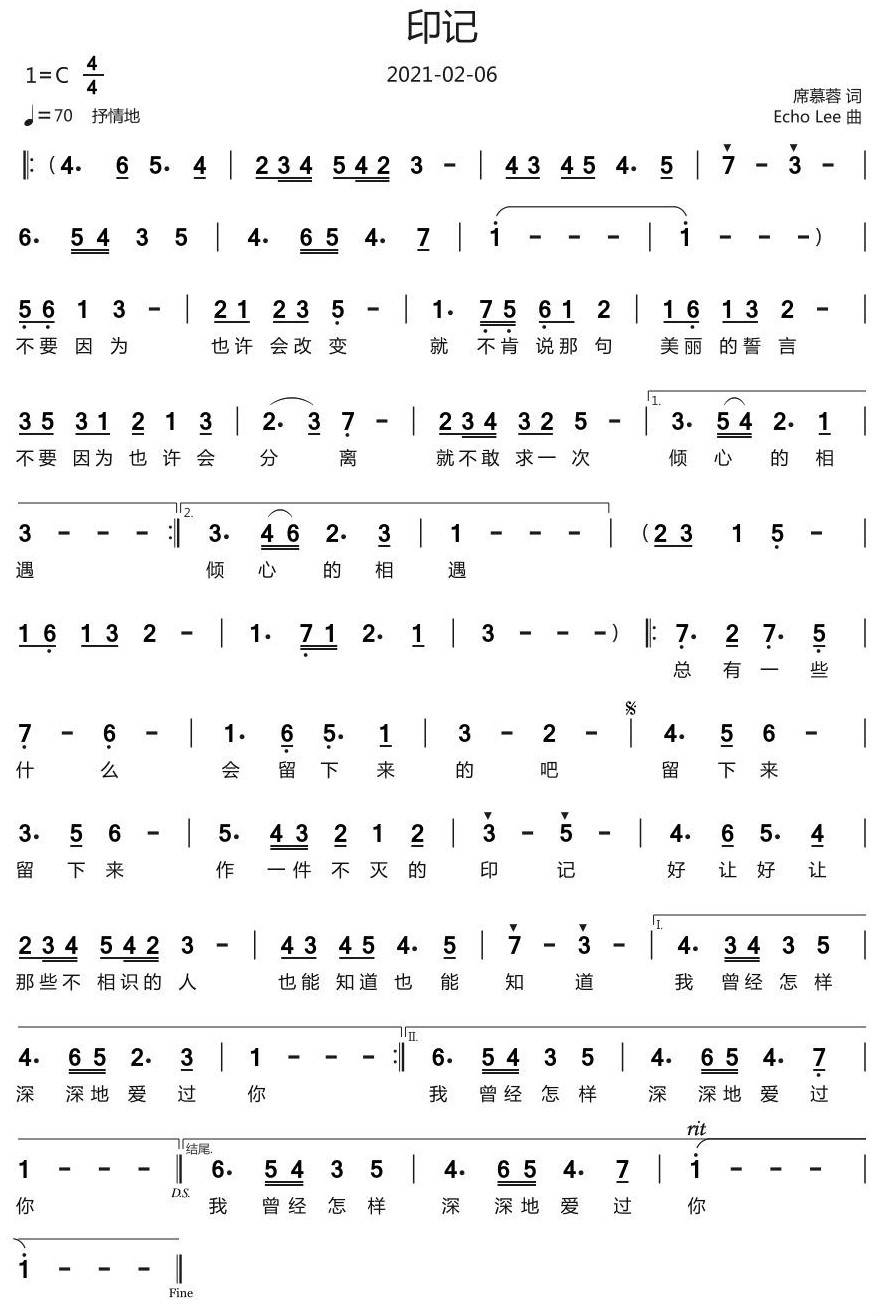
\includegraphics[width=0.9\textwidth]{rpi400/20210206印记.jpg}

\chapter{西游记}
\section{兒女情}                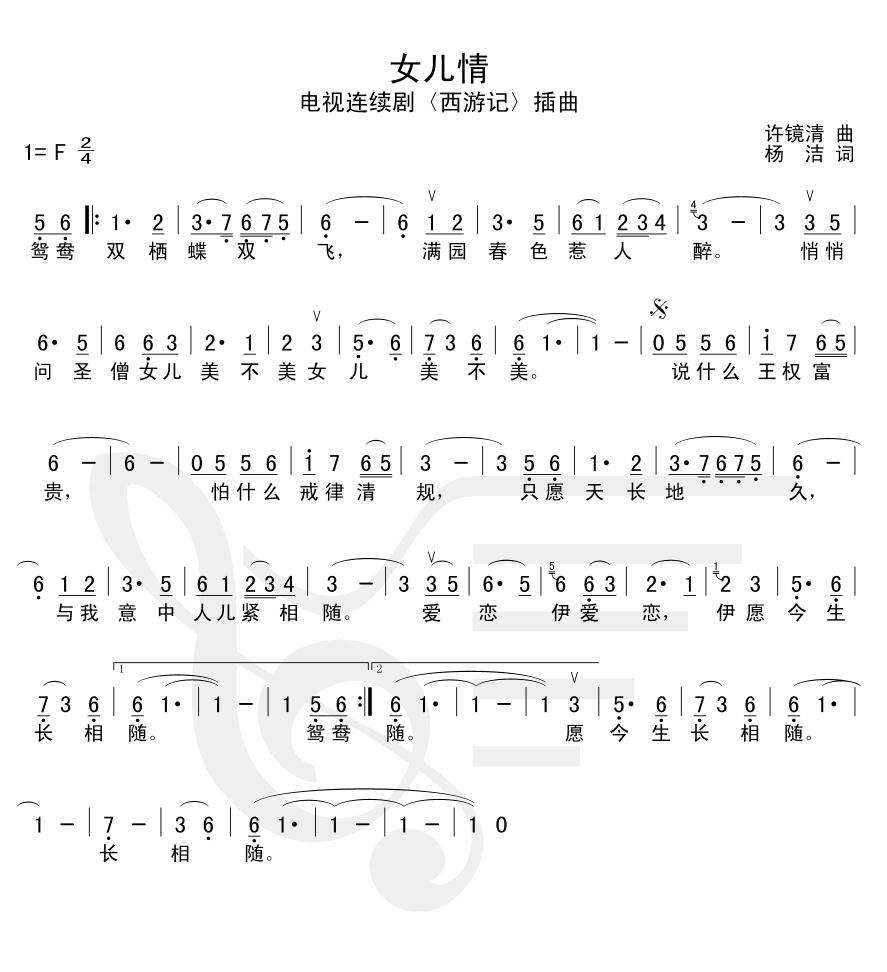
\includegraphics[width=\textwidth]{dongxiao/西游记-儿女情}  
\section{敢问路在何方}          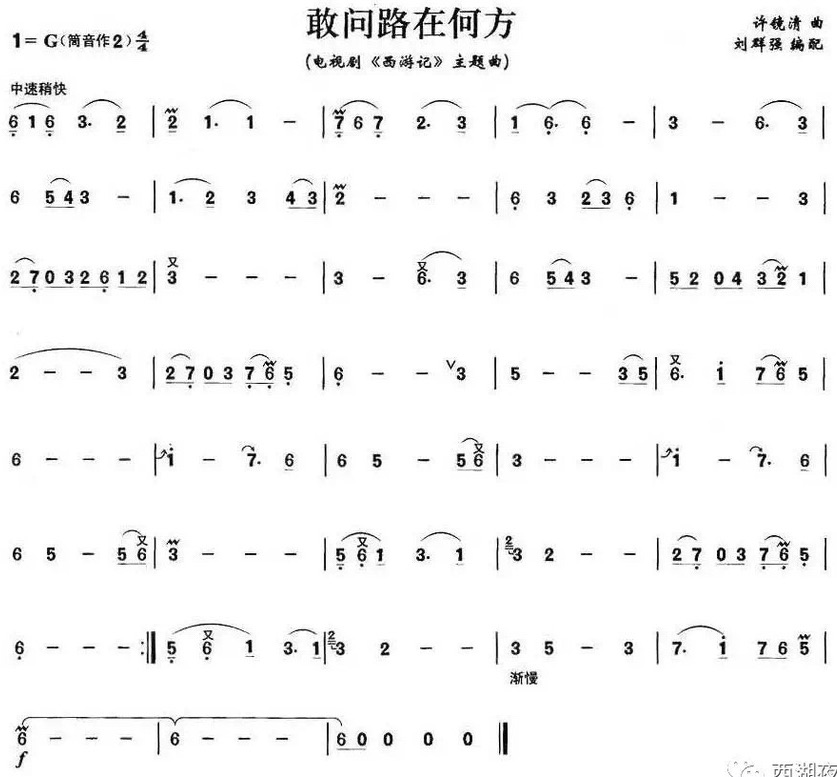
\includegraphics[width=\textwidth]{dongxiao/20200819/西游记-敢问路在何方.jpeg}
\section{晴空月儿明} 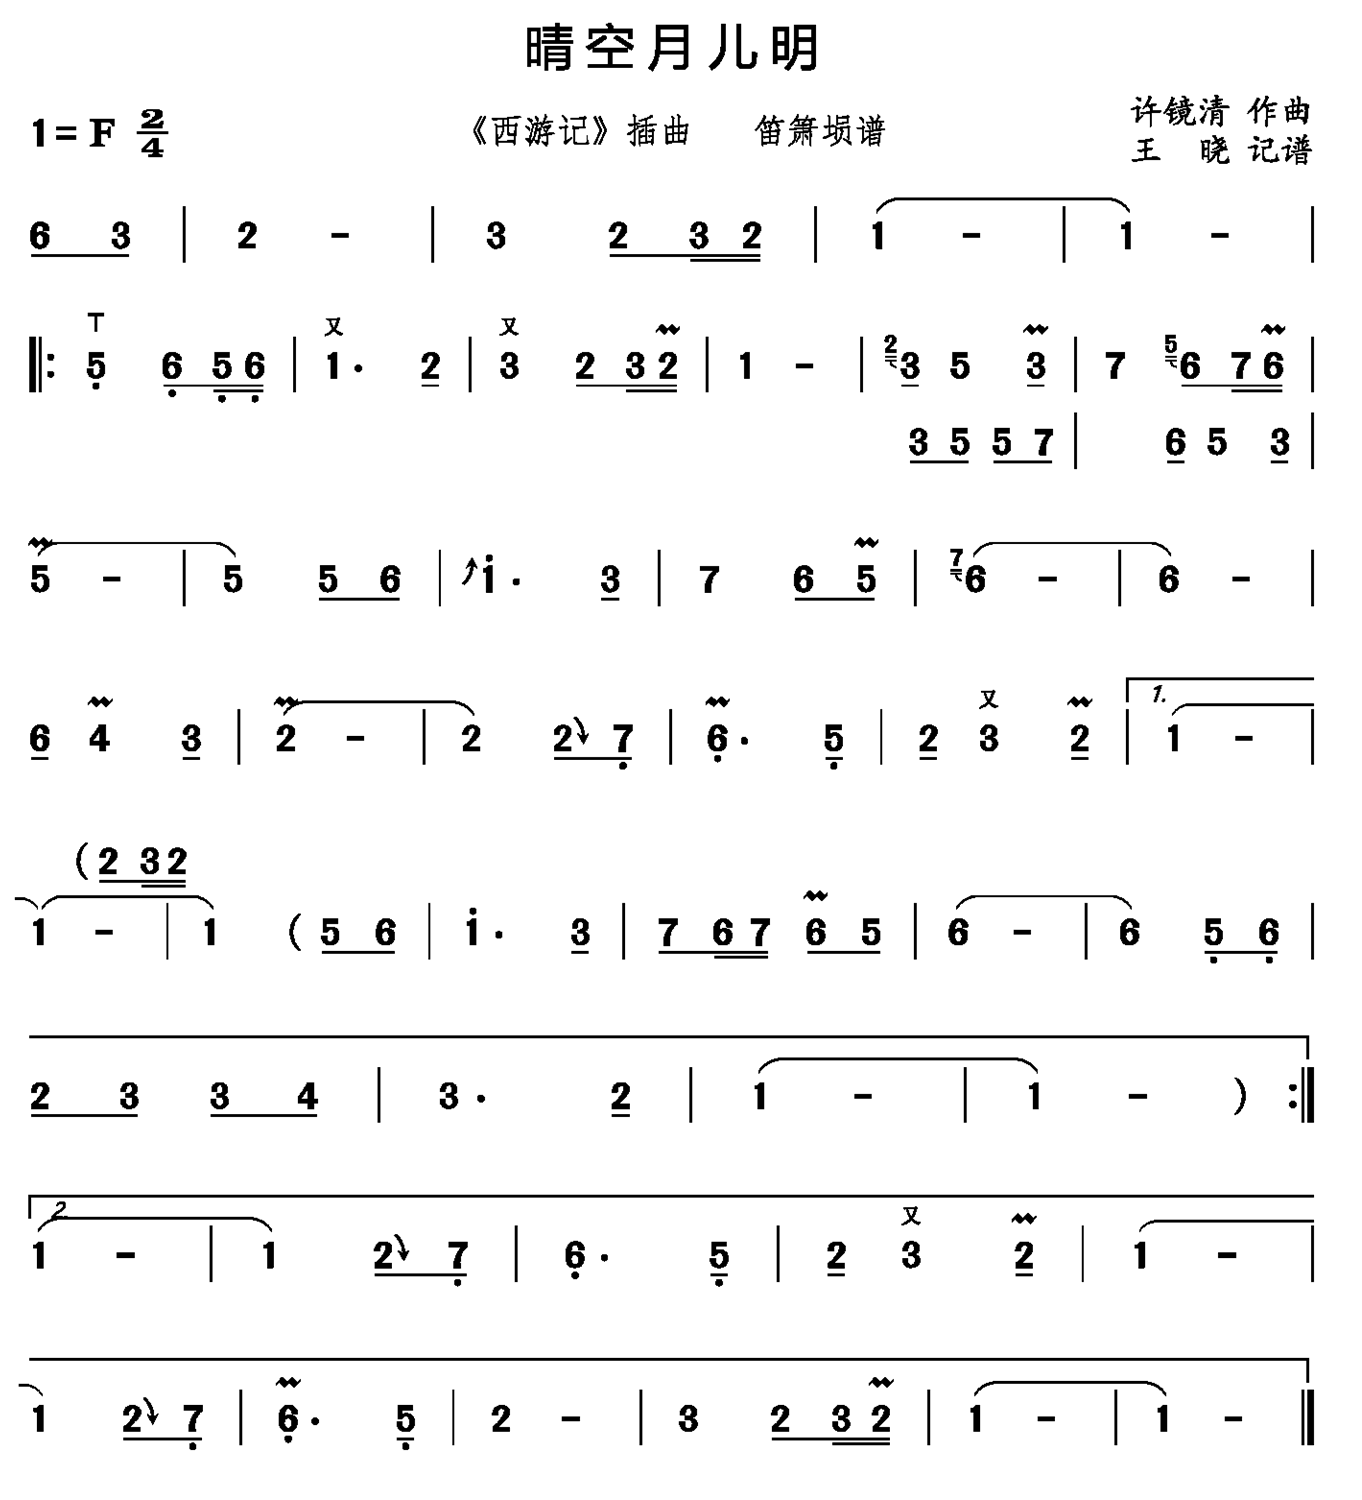
\includegraphics[width=\textwidth]{rpi400/20210206西游记晴空月儿明.png}
\section{青青菩提树} 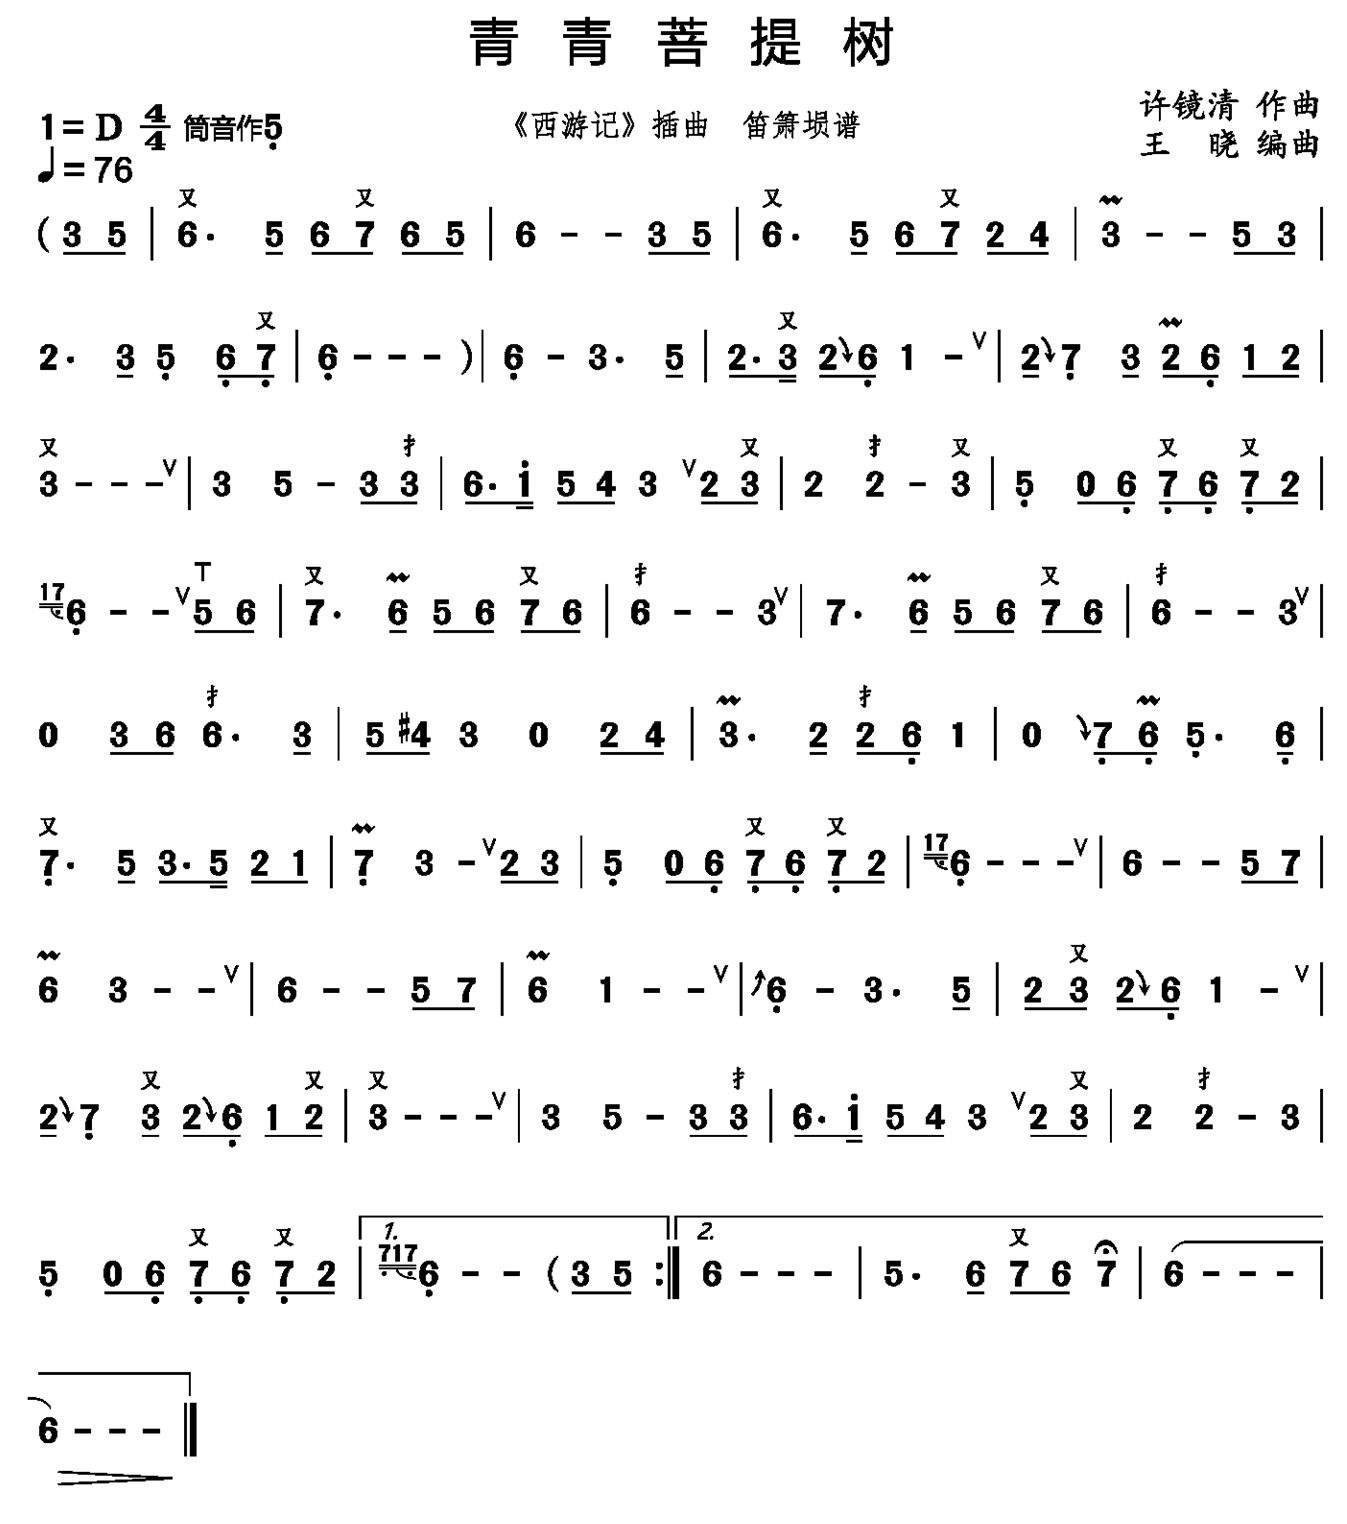
\includegraphics[width=\textwidth]{rpi400/20210206西游记青青菩提树.png}
\section{相思}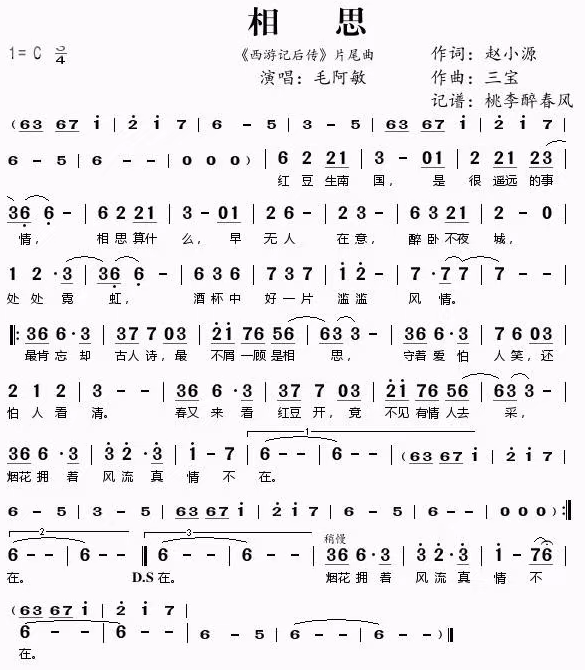
\includegraphics[width=\textwidth]{dongxiao/20200819/西游记-相思.png}

\chapter{诗经}
\section{关雎}      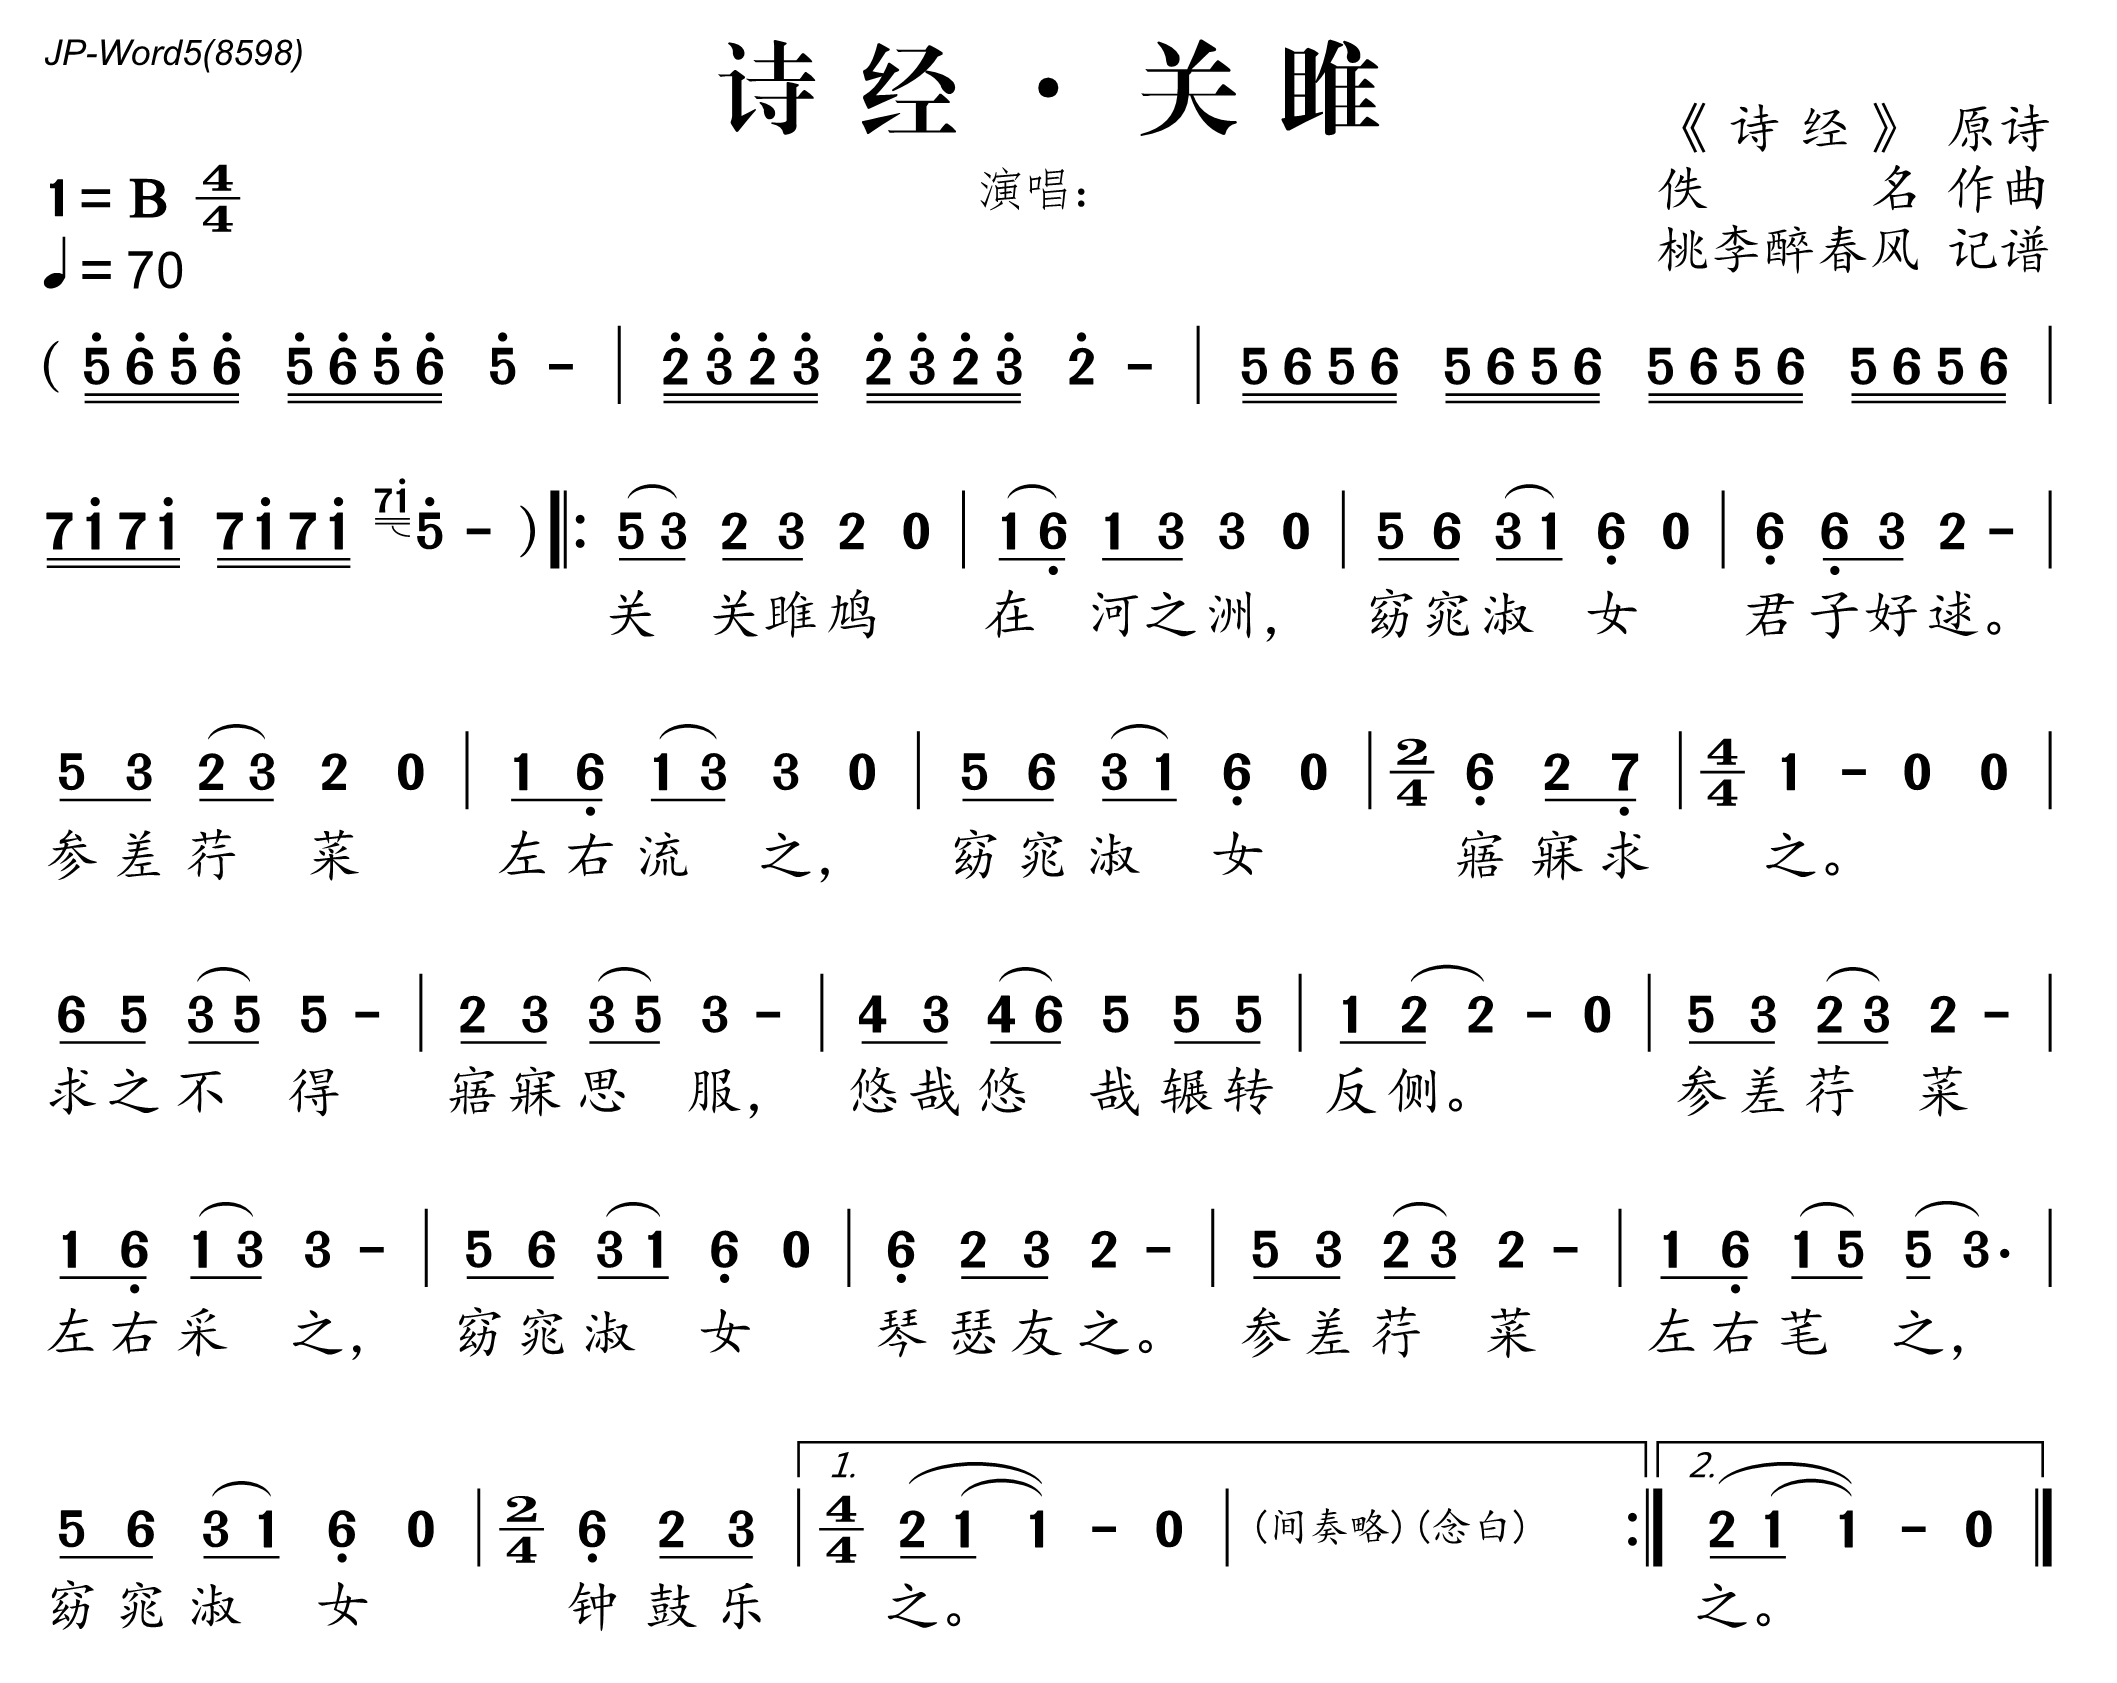
\includegraphics[width=\textwidth]{rpi400/20210124关雎.png}
\section{淇澳}      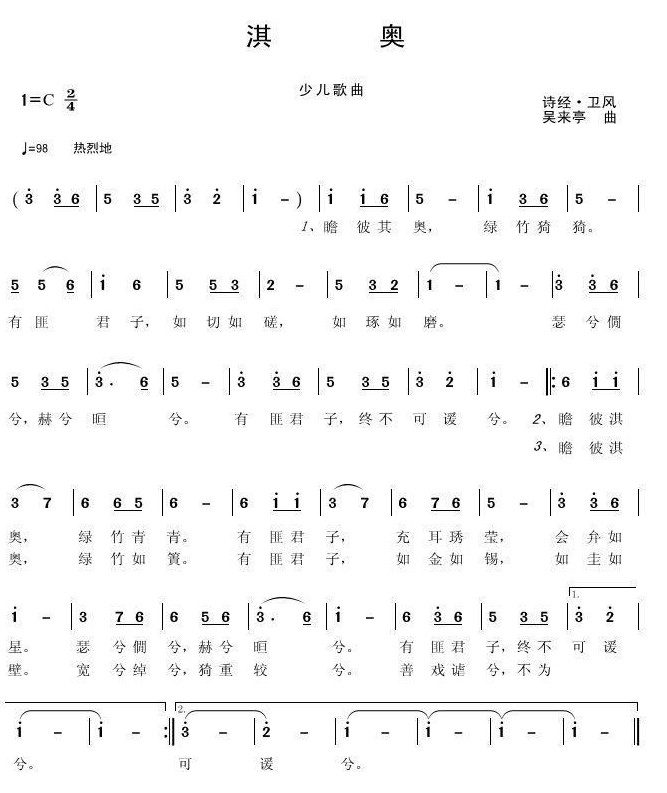
\includegraphics[width=\textwidth]{rpi400/20210123-淇澳.jpg}
\section{桃夭}      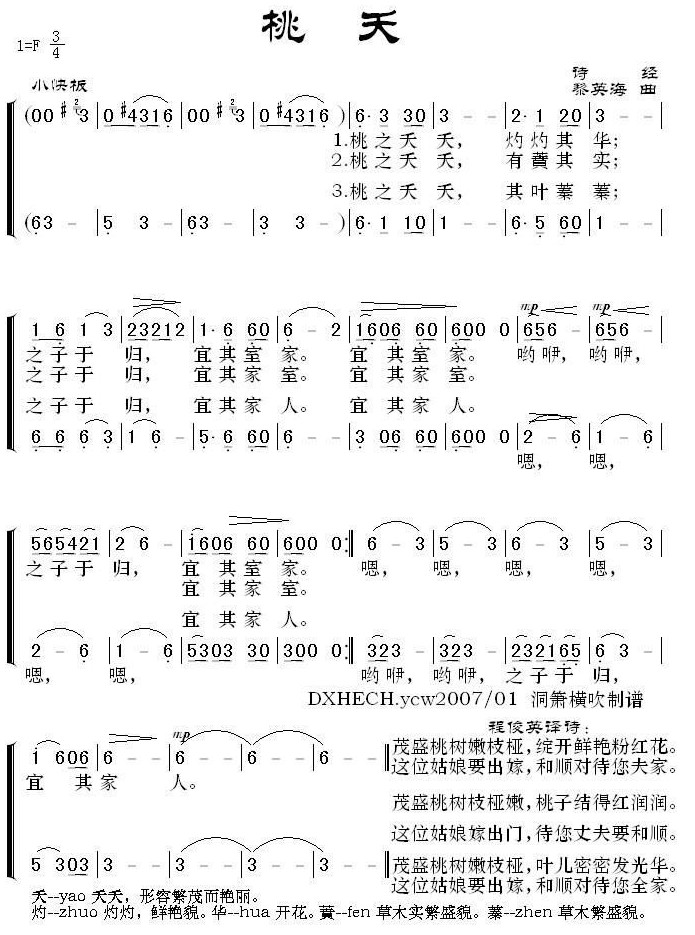
\includegraphics[width=0.9\textwidth]{rpi400/20210123-桃夭.jpg}
\section{\xpinyin*{葛覃}}      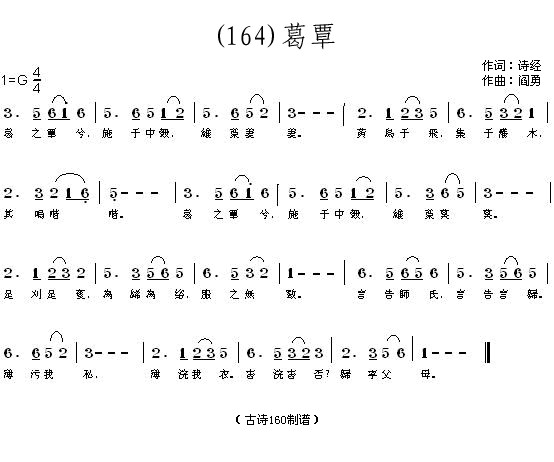
\includegraphics[width=\textwidth]{rpi400/20210123-葛覃.jpg}
\section{\xpinyin*{蒹葭}}      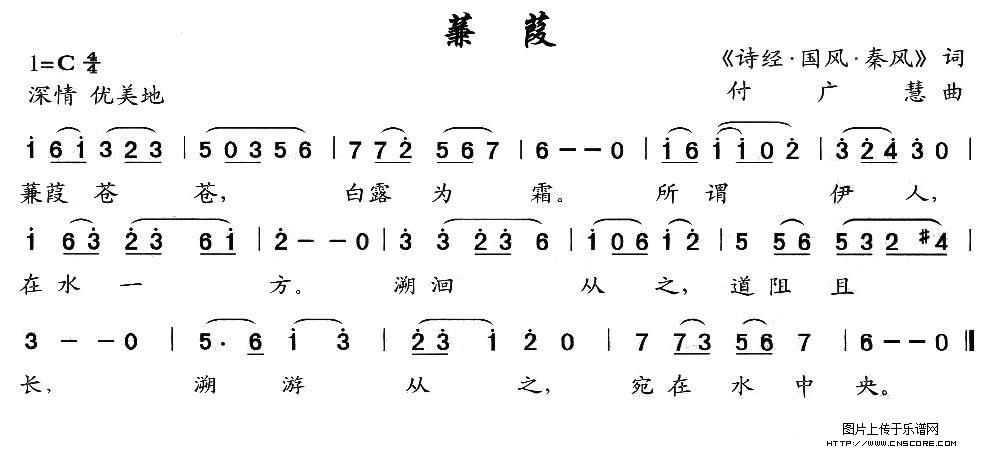
\includegraphics[width=\textwidth]{rpi400/20210123-蒹葭.jpg}
\section{蒹葭2}     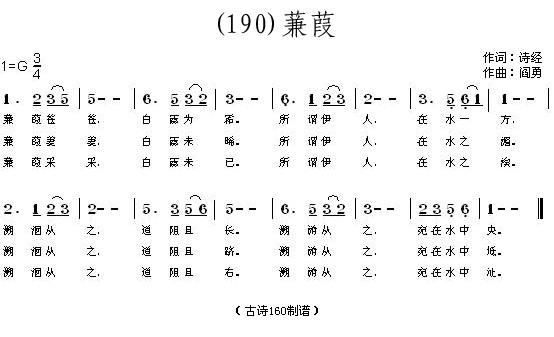
\includegraphics[width=\textwidth]{rpi400/20210123-蒹葭2.jpg}
\section{\xpinyin*{蜉蝣}}      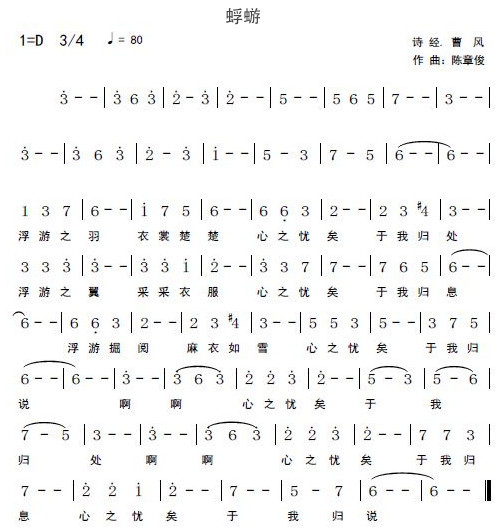
\includegraphics[width=\textwidth]{rpi400/20210123-蜉蝣.png}
\section{\xpinyin*{螽斯}}      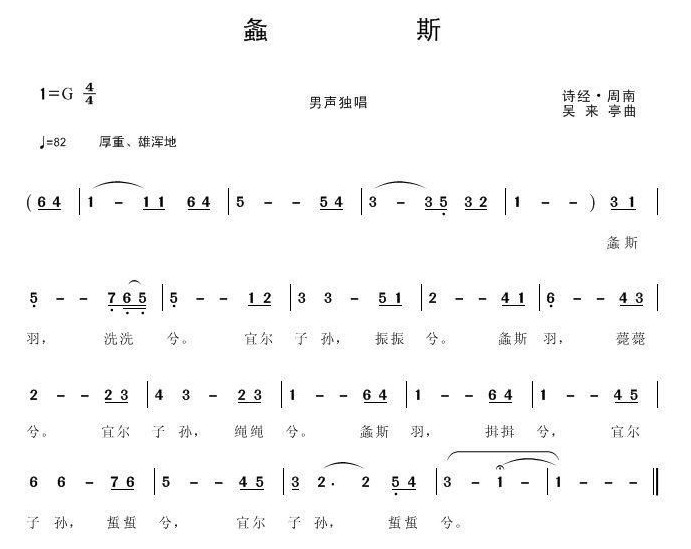
\includegraphics[width=\textwidth]{rpi400/20210123-螽斯.jpg}
\section{长发}      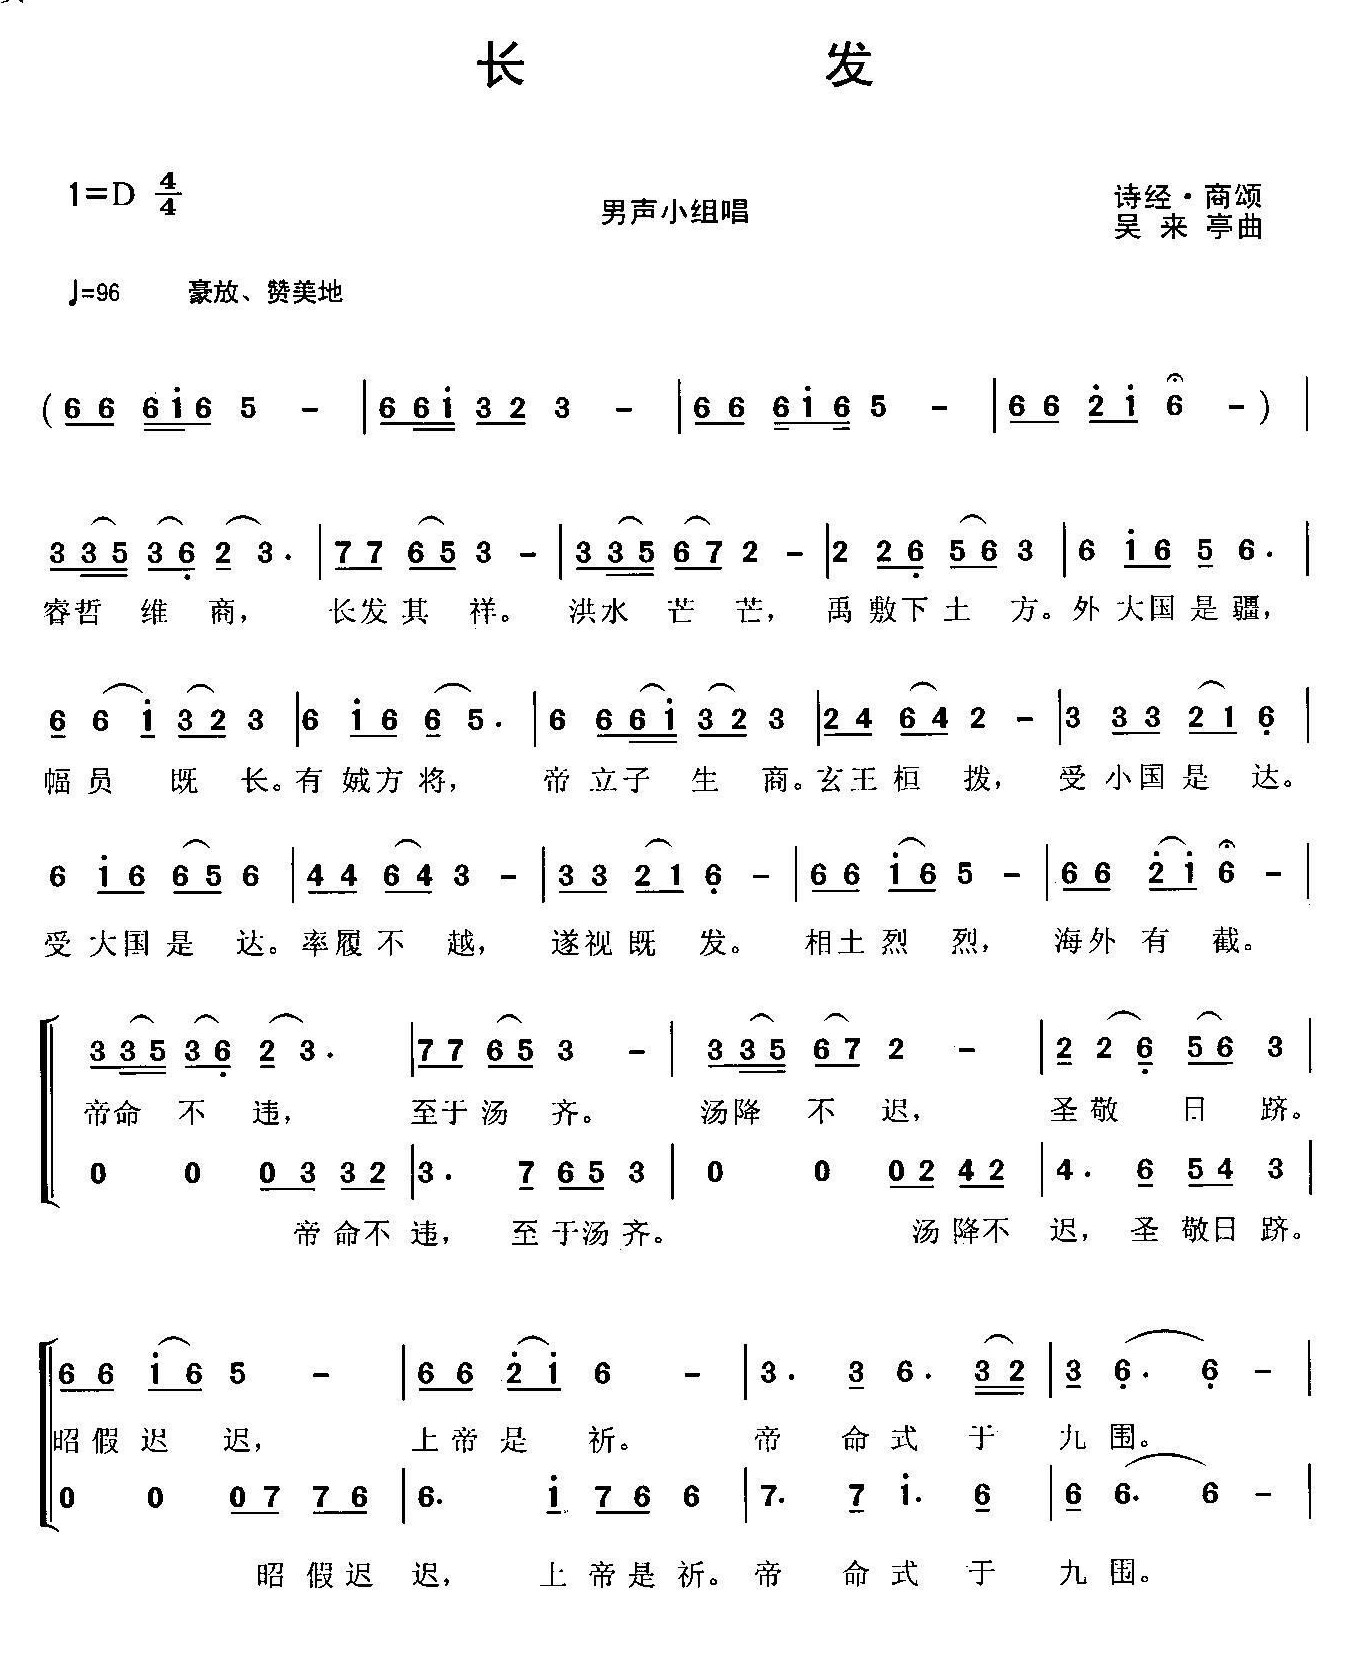
\includegraphics[width=\textwidth]{rpi400/20210123-长发.jpg}
\section{黍离}      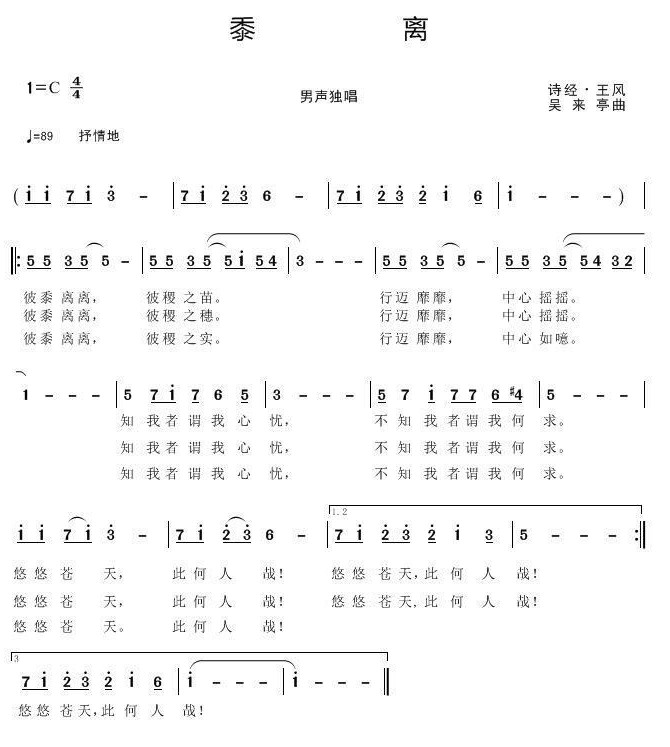
\includegraphics[width=\textwidth]{rpi400/20210123-黍离.jpg}
\section{鼓钟}      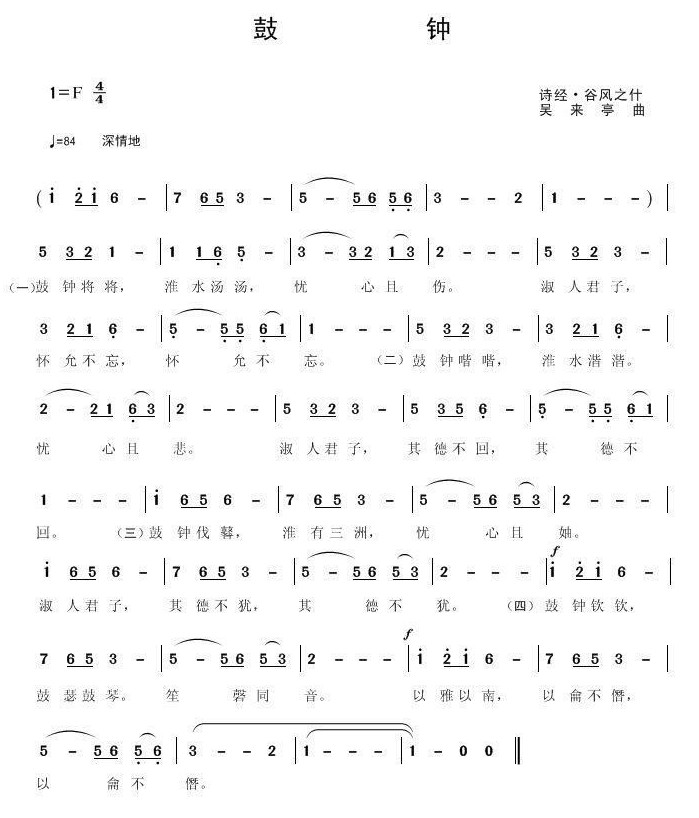
\includegraphics[width=\textwidth]{rpi400/20210123-鼓钟.jpg}
\section{越人歌}    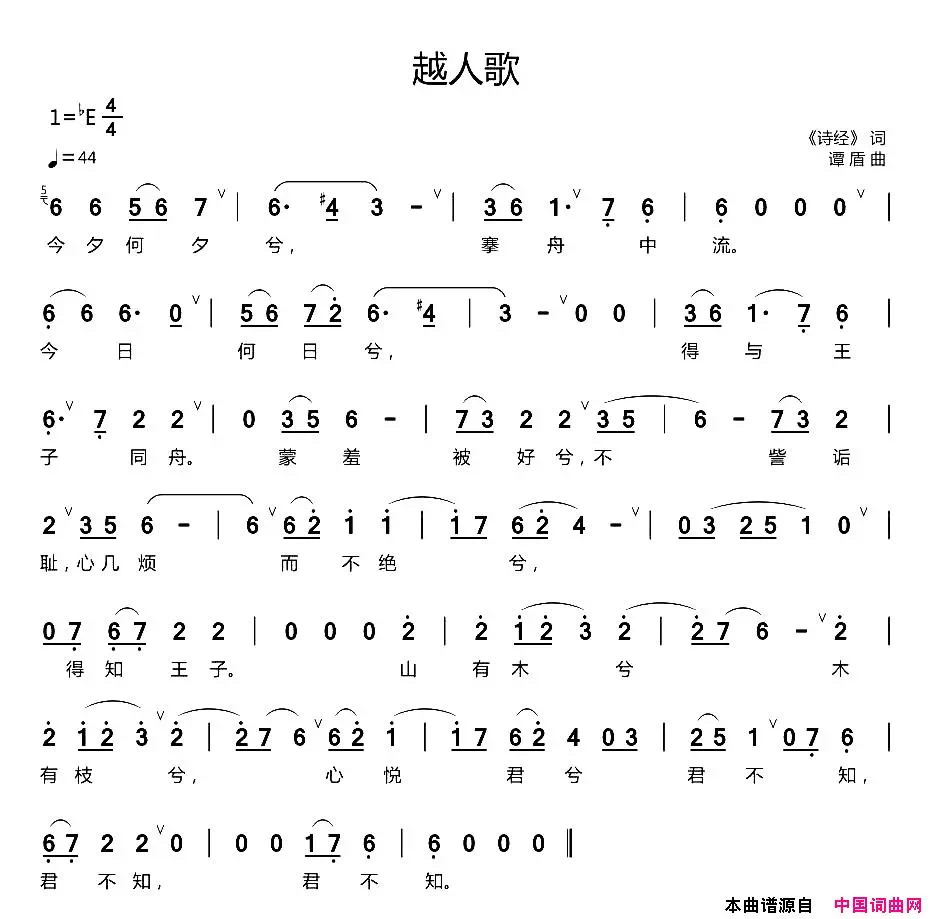
\includegraphics[width=\textwidth]{rpi400/20210123-越人歌.jpg}
\section{二子乘舟}  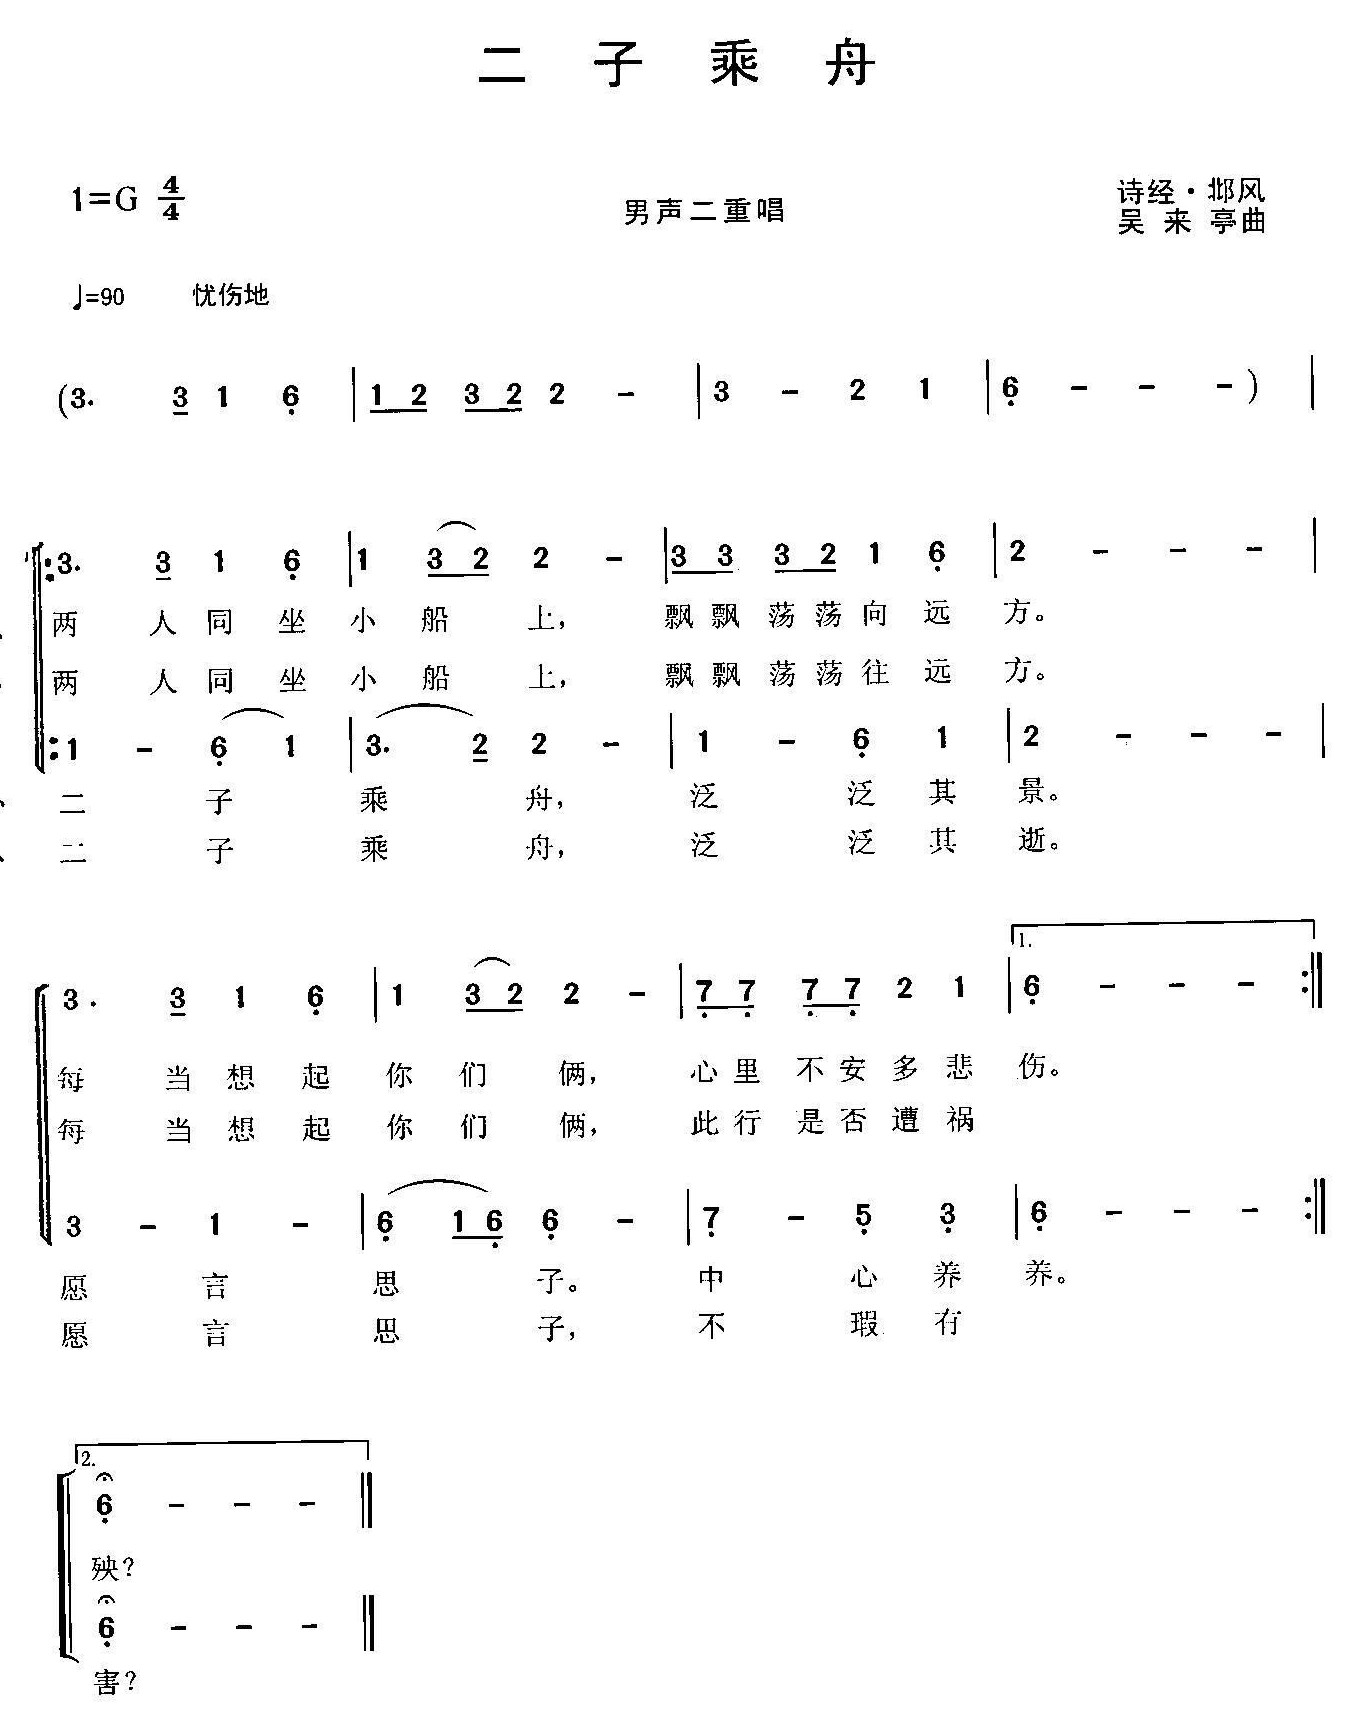
\includegraphics[width=\textwidth]{rpi400/20210123-二子乘舟.jpg}
\section{君子于役}  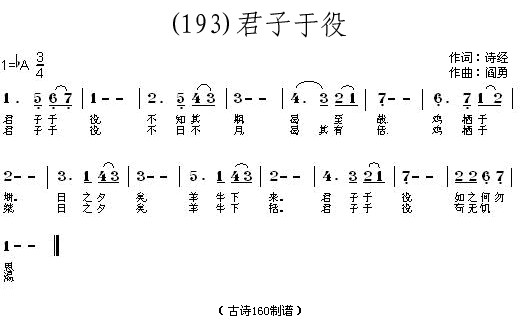
\includegraphics[width=\textwidth]{rpi400/20210123-君子于役.jpg}

\chapter{李叔同}
\section{忆儿时}    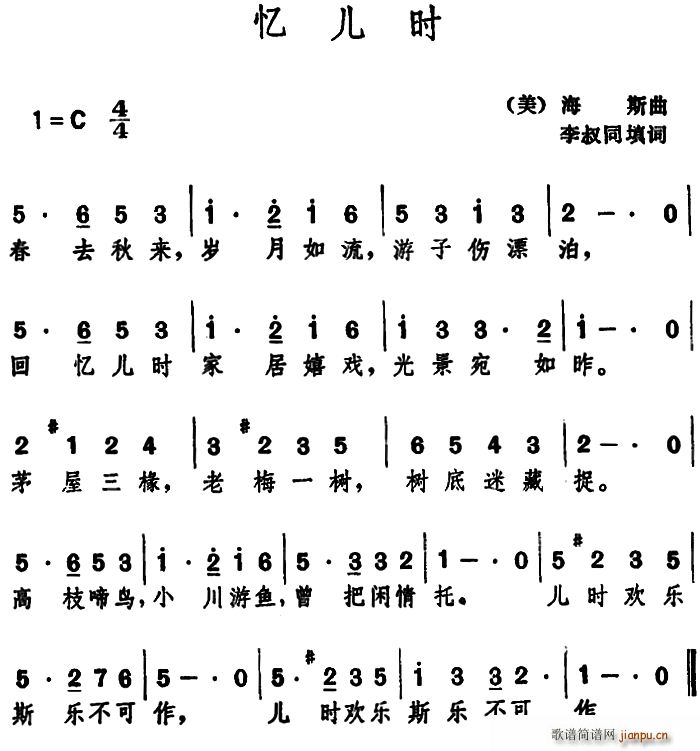
\includegraphics[width=\textwidth]{dongxiao/20200909-李叔同-忆儿时.jpg}  
\section{春游}      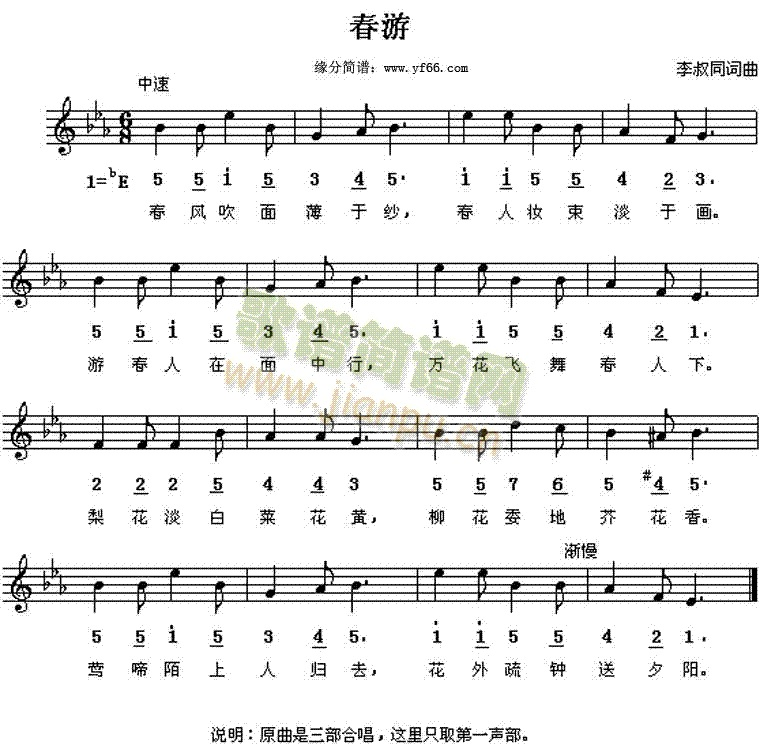
\includegraphics[width=\textwidth]{dongxiao/20200909-李叔同-春游.jpg} 
\section{早秋}      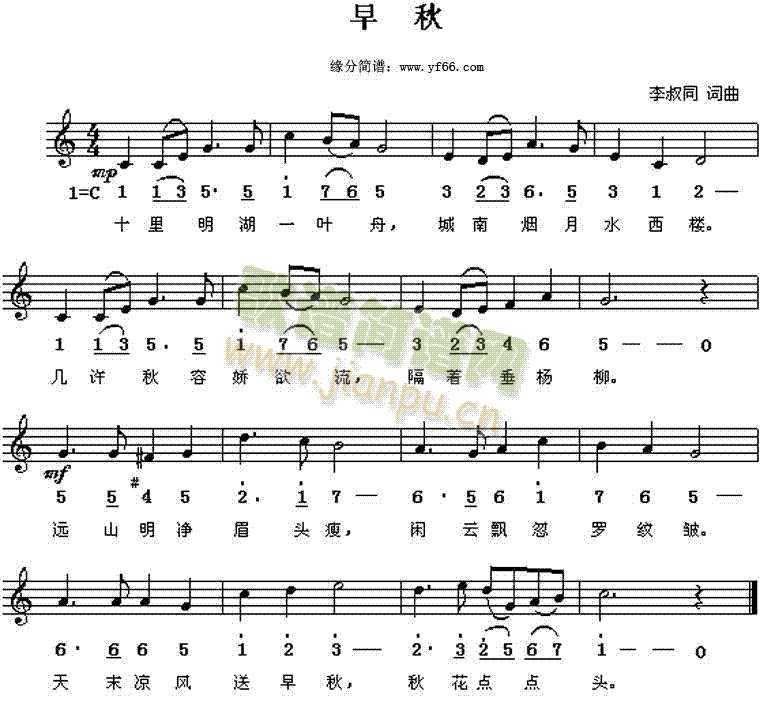
\includegraphics[width=\textwidth]{dongxiao/20200909-李叔同-早秋.jpg} 
\section{送别}      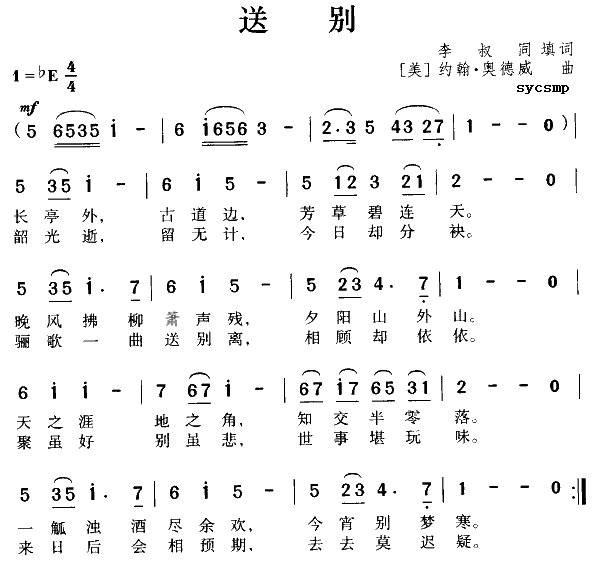
\includegraphics[width=\textwidth]{dongxiao/20200909-李叔同-送别.png} 

\chapter{王维}
\section{山中}      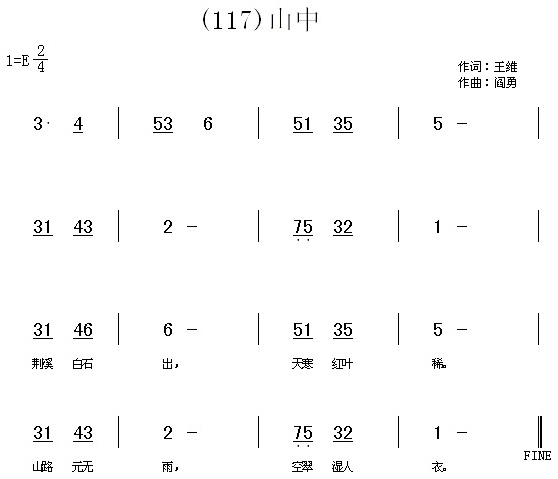
\includegraphics[width=\textwidth]{dongxiao/20200627-王维-山中.jpg}  
\section{山居秋暝}  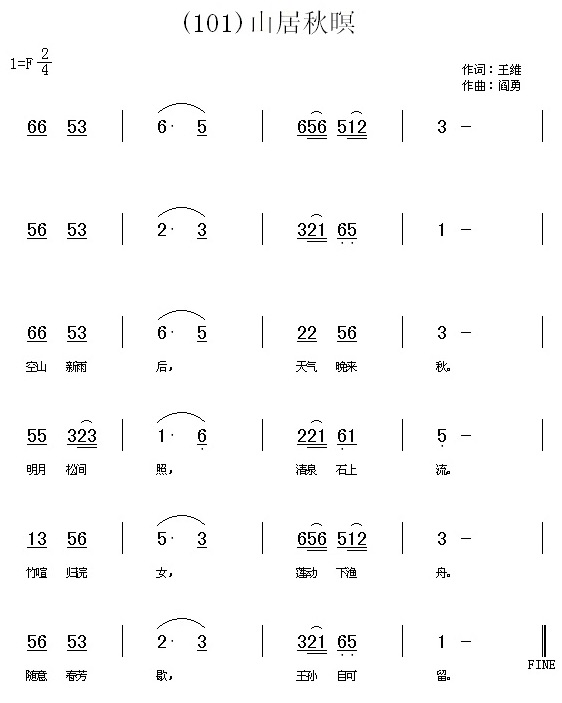
\includegraphics[width=\textwidth]{dongxiao/20200627-王维-山居秋暝.jpg} 
\section{辛夷坞}    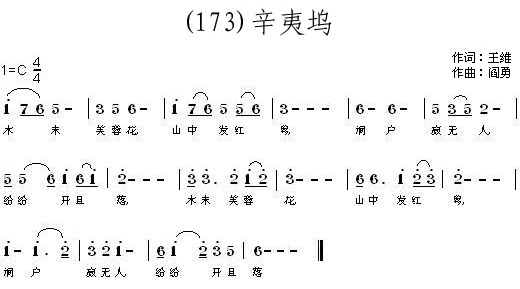
\includegraphics[width=\textwidth]{dongxiao/20200627-王维-辛夷坞.jpg} 
\section{红豆}      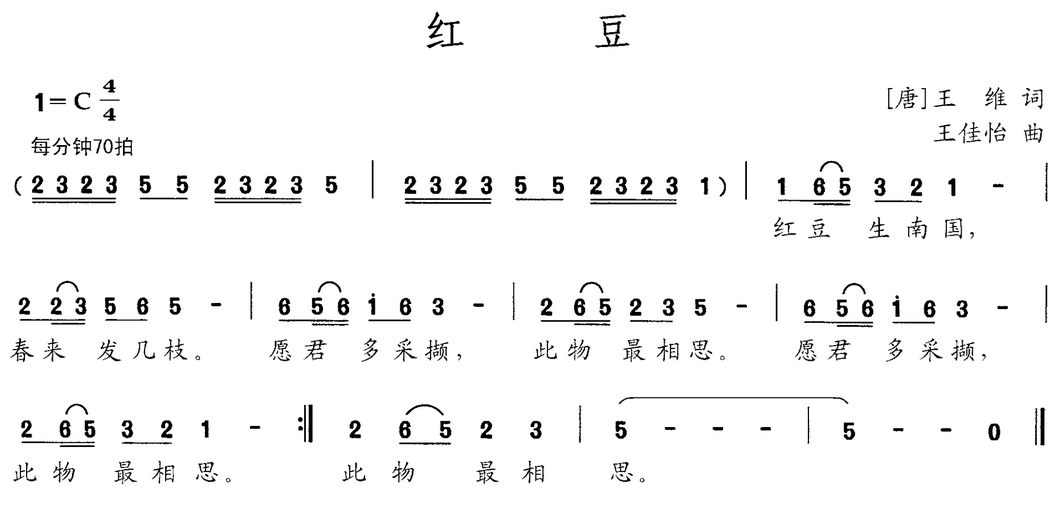
\includegraphics[width=\textwidth]{dongxiao/20200628-王维-红豆} 
\section{鸟鸣涧}    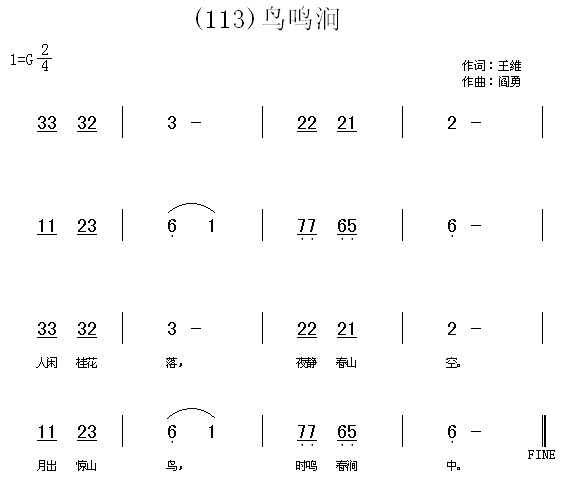
\includegraphics[width=\textwidth]{dongxiao/20200627-王维-鸟鸣涧}

\chapter{曹操}
\section{短歌行}    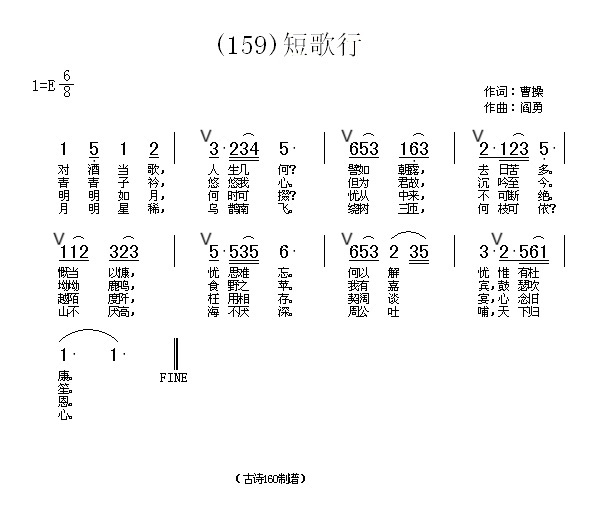
\includegraphics[width=\textwidth]{dongxiao/20200808-短歌行-曹操.jpg} 
\section{龟虽寿}    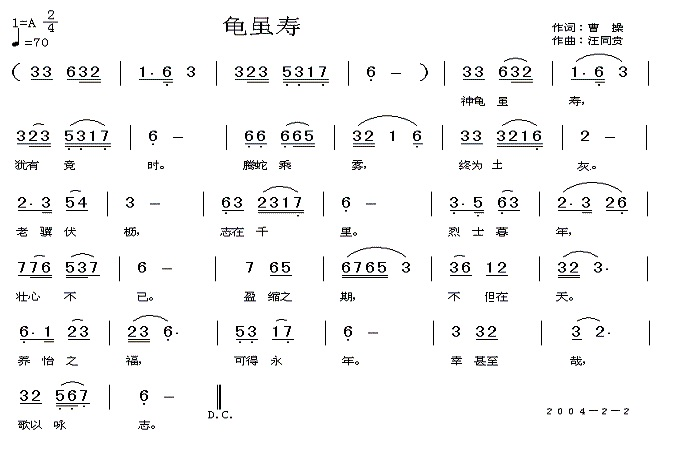
\includegraphics[width=\textwidth]{dongxiao/20200808-神龟虽寿-曹操.jpg}
\section{观沧海}    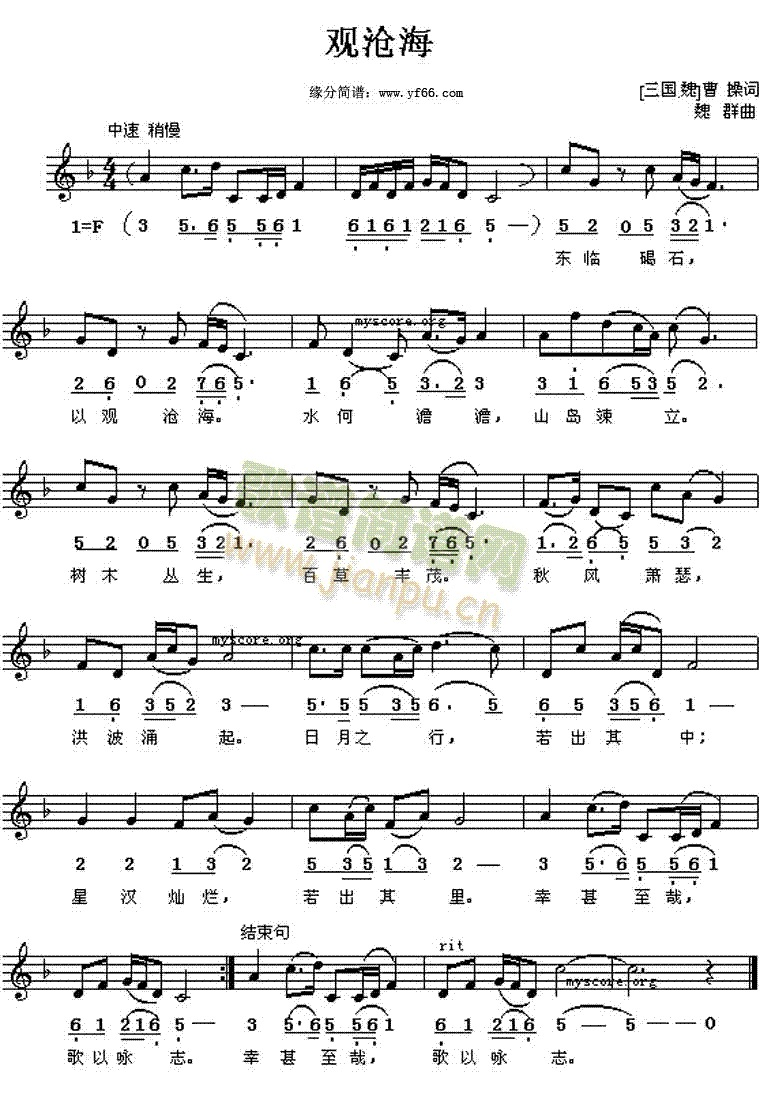
\includegraphics[width=0.9\textwidth]{dongxiao/20200808-观沧海-曹操.jpg}                             
\chapter{李健}
\section{一念一生} \includegraphics[width=0.85\textwidth]{rpi400/20210212李健一念一生.png}
\section{异乡人} \includegraphics[width=0.9\textwidth]{rpi400/20210212李健异乡人.png}
\section{日落之前} \includegraphics[width=0.9\textwidth]{rpi400/20210212李健日落之前.png}
\section{月光} \includegraphics[width=0.9\textwidth]{rpi400/20210212李健月光.jpg}
\section{沧海轻舟} \includegraphics[width=0.9\textwidth]{rpi400/20210212李健沧海轻舟.jpg}
\section{谢谢你} \includegraphics[width=0.9\textwidth]{rpi400/20210212李健谢谢你.png}
\section{风吹黄昏} \includegraphics[width=0.9\textwidth]{rpi400/20210212李健风吹黄昏.png}

\chapter{好妹妹乐队}
\section{南来的風}  \includegraphics[width=\textwidth]{dongxiao/20200516-好妹妹-南来的风.jpg} 
\section{冬}  \includegraphics[width=\textwidth]{dongxiao/20200516-好妹妹-冬.jpg}
\section{西窗的雨}  \includegraphics[width=\textwidth]{dongxiao/20200516-好妹妹-西窗的雨.jpg} 
\section{你曾是少年}  \includegraphics[width=0.9\textwidth]{dongxiao/20200516-好妹妹-你曾是少年.jpg} 
\section{风又吹走了}  \includegraphics[width=\textwidth]{dongxiao/20200516-好妹妹-风又吹走了.jpg} 
\section{送你一朵山茶花}  \includegraphics[width=\textwidth]{dongxiao/20200516-好妹妹-送你一朵山茶花.jpg}


\chapter{苏轼}
\section{黄州定慧院寓居作}          \includegraphics[width=\textwidth]{dongxiao/20200627-苏轼-黄州定慧院寓居作.jpg} 
\section{定风波}                    \includegraphics[width=\textwidth]{dongxiao/20200411-定风波.jpg}
\section{蝶恋花-春景}               \includegraphics[width=\textwidth]{dongxiao/20200411-蝶恋花-春景.jpg}
\section{六月二十七日望湖楼醉书}    \includegraphics[width=\textwidth]{dongxiao/20200627-苏轼-六月二十七日望湖楼醉书.jpg} 
\section{江城子}                    \includegraphics[width=\textwidth]{dongxiao/20200627-苏轼-江城子.jpg} 
\section{花影}                      \includegraphics[width=\textwidth]{dongxiao/20200627-苏轼-花影.jpg} 
\section{饮湖上初晴后雨}            \includegraphics[width=\textwidth]{dongxiao/20200627-苏轼-饮湖上初晴后雨.jpg} 
\section{明月几时有}                \includegraphics[width=\textwidth]{dongxiao/20200411-明月几时有.jpg}
\section{十年生死两茫茫}            \includegraphics[width=\textwidth]{dongxiao/20200627-苏轼-十年生死两茫茫.jpg} 
\section{念奴娇赤壁怀古}            \includegraphics[width=\textwidth]{dongxiao/20200801-苏轼-念奴娇赤壁怀古}
\section{花褪残红青杏小}            \includegraphics[width=\textwidth]{dongxiao/20200801-苏轼-花褪残红青杏小} 
\section{大江东去}                  \includegraphics[width=\textwidth]{rpi400/20201230大江东去.jpg}
\section{明月几时有}                \includegraphics[width=\textwidth]{rpi400/20201230明月几时有.jpg}
\section{江城子}                    \includegraphics[width=\textwidth]{rpi400/20201230江城子.jpg}
\section{赤壁怀古}                  \includegraphics[width=\textwidth]{rpi400/20201230赤壁怀古.jpg}

\chapter{李清照}
\section{如梦令}        \includegraphics[width=\textwidth]{dongxiao/20200808-如梦令-李清照.jpg}
\section{醉花阴}        \includegraphics[width=\textwidth]{dongxiao/20200808-醉花阴-李清照.jpg} 
\section{常记溪亭日暮}  \includegraphics[width=\textwidth]{dongxiao/20200808-常记溪亭日暮-李清照.jpg}
\section{昨夜雨疏风骤}  \includegraphics[width=\textwidth]{dongxiao/20200808-昨夜雨疏风骤-李清照.jpg}    
   
\chapter{杜甫}
\section{忆昔}          \includegraphics[width=\textwidth]{dongxiao/20200808-忆昔-杜甫.jpg} 
\section{春夜喜雨}      \includegraphics[width=\textwidth]{dongxiao/20200808-春夜喜雨-杜甫.jpg}
\section{春望}          \includegraphics[width=\textwidth]{dongxiao/20200808-春望-杜甫.jpg}
\section{赠花卿}        \includegraphics[width=\textwidth]{dongxiao/20200808-赠花卿-杜甫.jpg}    
\section{月夜}          \includegraphics[width=\textwidth]{dongxiao/20200808-月夜-杜甫.jpg}                     
\section{江畔独步寻花}  \includegraphics[width=\textwidth]{dongxiao/20200808-江畔独步寻花-杜甫.jpg}   

\chapter{李白}
\section{忆秦娥}    \includegraphics[width=\textwidth]{dongxiao/20200808-忆秦娥-李白.jpg} 
\section{怨情}      \includegraphics[width=\textwidth]{dongxiao/20200808-怨情-李白.jpg}
\section{春思}      \includegraphics[width=\textwidth]{dongxiao/20200808-春思-李白.jpg}
\section{古朗月行}  \includegraphics[width=\textwidth]{dongxiao/20200808-古朗月行-李白.jpg}    
\section{月下独酌}  \includegraphics[width=0.95\textwidth]{dongxiao/20200808-月下独酌-李白.jpg} 
\section{秋浦歌}    \includegraphics[width=\textwidth]{dongxiao/20200808-秋浦歌-李白.jpg}
\section{独坐敬亭山}\includegraphics[width=\textwidth]{dongxiao/20200808-独坐敬亭山-李白.jpg}
\section{望庐山瀑布}\includegraphics[width=\textwidth]{dongxiao/20200808-望庐山瀑布-李白.jpg}
\section{美人怨}    \includegraphics[width=\textwidth]{dongxiao/20200808-美人怨-李白.jpg}
\section{菩萨蛮}    \includegraphics[width=\textwidth]{dongxiao/20200808-菩萨蛮-李白.jpg}
      
\chapter{陆游}
\section{示儿}      \includegraphics[width=\textwidth]{dongxiao/20200808-示儿-陆游.jpg} 
\section{红酥手}    \includegraphics[width=\textwidth]{dongxiao/20200808-红酥手-陆游.jpg}
\section{钗头凤}    \includegraphics[width=0.7\textwidth]{dongxiao/20200808-钗头凤-陆游.jpg}                             
\section{题临安邸}  \includegraphics[width=\textwidth]{dongxiao/20200808-题临安邸-陆游.jpg}                             
 
\chapter{古诗}
\section{乞巧(唐,林杰)}      \includegraphics[width=\textwidth]{dongxiao/20200627-古诗-乞巧.jpg}     
\section{咏柳(唐,贺知章)}    \includegraphics[width=0.9\textwidth]{dongxiao/20200627-古诗-咏柳.jpg}   
\section{夜书所见(宋,叶绍翁)}\includegraphics[width=0.8\textwidth]{dongxiao/20200627-古诗-夜书所见.jpg}   
\section{春日(宋,朱熹)}      \includegraphics[width=0.8\textwidth]{dongxiao/20200627-古诗-春日.jpg}   
\section{望洞庭(唐,刘禹锡)}  \includegraphics[width=\textwidth]{dongxiao/20200627-古诗-望洞庭.jpg}   
\section{绝句(唐,杜甫)}      \includegraphics[width=0.8\textwidth]{dongxiao/20200627-古诗-杜甫-绝句.jpg}   
\section{秋思(唐,张籍)}      \includegraphics[width=\textwidth]{dongxiao/20200627-古诗-秋思.jpg}   
\section{草(唐,白居易)}      \includegraphics[width=0.9\textwidth]{dongxiao/20200627-古诗-草.jpg}   
\section{赠汪伦(唐,李白)}    \includegraphics[width=0.9\textwidth]{dongxiao/20200627-古诗-赠汪伦.jpg}   
\section{已亥杂诗(清,龚自珍)}\includegraphics[width=\textwidth]{dongxiao/20200627-古诗-龚自珍-已亥杂诗.jpg}   
\section{枫桥夜泊}              \includegraphics[width=\textwidth]{dongxiao/20200808-枫桥夜泊-昆曲.jpg}   
\section{枫桥夜泊2}             \includegraphics[width=\textwidth]{dongxiao/20200808-枫桥夜泊-张继.jpg}  
                            
  
\chapter{日本歌譜}
\section{樱花}      \includegraphics[width=\textwidth]{dongxiao/日本-樱花.jpg}  
\section{风的大地}  \includegraphics[width=\textwidth]{dongxiao/20200628-日本-风的大地}  
\section{黎明之歌}  \includegraphics[width=\textwidth]{dongxiao/20200628-日本-黎明之歌}  
	
\chapter{杂录(一)}
\section{长城谣}    \includegraphics[width=\textwidth]{dongxiao/20200711-长城谣.jpg}
\section{有所思}    \includegraphics[width=\textwidth]{dongxiao/20200710-有所思}
\section{西湖春}    \includegraphics[width=\textwidth]{dongxiao/20200711-西湖春.jpg}
\section{茉莉花}    \includegraphics[width=\textwidth]{dongxiao/20200711-茉莉花.jpg}
\section{苏武牧羊}  \includegraphics[width=\textwidth]{dongxiao/20200711-苏武牧羊.jpeg}
\section{关山月}    \includegraphics[width=\textwidth]{dongxiao/20200411-清平乐-关山月.jpg}
\section{清平乐-春归何处}\includegraphics[width=\textwidth]{dongxiao/20200411-清平乐-春归何处.jpg}
\section{清平乐-晏殊词}\includegraphics[width=\textwidth]{dongxiao/20200411-清平乐-晏殊.jpg}
\section{时间都去哪儿了}\includegraphics[width=\textwidth]{dongxiao/20200411-时间都去哪儿了.jpg} 
\section{城市很静}  \includegraphics[width=\textwidth]{dongxiao/20200402-城市很静} 
\section{玉楼春}    \includegraphics[width=\textwidth]{dongxiao/20200323玉楼春.jpg}
\section{墨香-长安曲}\includegraphics[width=0.9\textwidth]{dongxiao/20200323墨香-长安曲.jpg} 
\section{思美人兮}  \includegraphics[width=\textwidth]{dongxiao/20200402-思美人.jpg}
\section{無羈}      \includegraphics[width=\textwidth]{dongxiao/20201231-無羈} 
\section{心經}      \includegraphics[width=\textwidth]{dongxiao/20201231-心经} 
\section{失魂引}    \includegraphics[width=0.9\textwidth]{rpi400/20201226失魂引.png}
\section{云愁雨恨}  \includegraphics[width=0.9\textwidth]{rpi400/20201226云愁雨恨.png}
\section{柳林坡}    \includegraphics[width=\textwidth]{dongxiao/20201231-柳林坡}
\section{殘月}      \includegraphics[width=\textwidth]{dongxiao/20201231-残月}
\section{漢江殘雪}  \includegraphics[width=0.9\textwidth]{dongxiao/20201231-汉江残雪} 
\section{煙雨}      \includegraphics[width=0.95\textwidth]{dongxiao/20201231-烟雨}
\section{聞笛碎念}  \includegraphics[width=0.95\textwidth]{dongxiao/20201231-闻地碎念} 
\section{青青菩提樹}\includegraphics[width=\textwidth]{dongxiao/20201231-青青菩提树}
\section{七步诗}    \includegraphics[width=\textwidth]{dongxiao/20200808-七步诗-戴与吾.jpg}
\section{七步诗2}   \includegraphics[width=\textwidth]{dongxiao/20200808-七步诗-曹植.jpg}
\section{乌衣巷}    \includegraphics[width=\textwidth]{dongxiao/20200808-乌衣巷-刘禹锡.jpg}
\section{竹石}      \includegraphics[width=\textwidth]{dongxiao/20200808-竹石-郑燮.jpg}
\section{九曲黄河万里沙}\includegraphics[width=\textwidth]{dongxiao/20200808-浪淘沙-九曲黄河万里沙-刘禹锡.jpg}
\section{浪淘沙}    \includegraphics[width=0.95\textwidth]{dongxiao/20200808-浪淘沙-欧阳修.jpg}
\section{一壶紫笋为谁香}\includegraphics[width=0.9\textwidth]{dongxiao/20200901-一壶紫笋为谁香.jpeg} 
\section{思乡的梦里} \includegraphics[width=\textwidth]{dongxiao/20200901-思乡的梦里.jpeg}
\section{情醉西湖} \center\includegraphics[width=0.8\textwidth]{dongxiao/20200901-情醉西湖.jpeg}
\section{旧日欢颜}  \includegraphics[width=0.95\textwidth]{dongxiao/20200901-旧日欢颜.jpeg} 
\section{梵声万里}  \includegraphics[width=\textwidth]{dongxiao/20200901-梵声万里.jpeg}
\section{楼台}      \includegraphics[width=0.9\textwidth]{dongxiao/20200901-楼台.jpeg}
\section{相思河}    \includegraphics[width=\textwidth]{dongxiao/20200901-相思河.jpeg}
\chapter{杂录(二)}
\section{沉醉曹山}  \includegraphics[width=0.95\textwidth]{dongxiao/20200808-沉醉曹山.jpg}
\section{残月}      \includegraphics[width=0.95\textwidth]{dongxiao/20200909-残月.jpg}
\section{水岸风堤}  \includegraphics[width=0.95\textwidth]{dongxiao/20200909-水岸风堤.jpg}
\section{烟雨}      \includegraphics[width=0.95\textwidth]{dongxiao/20200909-烟雨.jpg}
\section{菩萨蛮.箫声咽}\includegraphics[width=0.95\textwidth]{dongxiao/20200909-箫声咽-菩萨蛮.jpg}
\section{云门夜雨}\includegraphics[width=0.88\textwidth]{dongxiao/20200819/云门夜雨.jpeg}
\section{佚名曲}\includegraphics[width=0.95\textwidth]{dongxiao/20200819/佚名曲.png}
\section{佛上店}\includegraphics[width=0.95\textwidth]{dongxiao/20200819/佛上店.png}
\section{倩女幽魂}\includegraphics[width=0.95\textwidth]{dongxiao/20200819/倩女幽魂.jpeg}
\section{凉凉}\includegraphics[width=0.95\textwidth]{dongxiao/20200819/凉凉.jpeg}
\section{几多愁}\includegraphics[width=0.95\textwidth]{dongxiao/20200819/几多愁.jpeg}
\section{刹那一永恒}\includegraphics[width=0.95\textwidth]{dongxiao/20200819/刹那-永恒.png}
\section{匆匆那年}\includegraphics[width=\textwidth]{dongxiao/20200819/匆匆那年.jpeg}
\section{半壶纱}\includegraphics[width=\textwidth]{dongxiao/20200819/半壶纱.jpeg}
\section{古境幽刹}\includegraphics[width=0.95\textwidth]{dongxiao/20200819/古刹幽境.jpeg}
\section{大话西游-插曲}\includegraphics[width=\textwidth]{dongxiao/20200819/大话西游插曲.jpeg}
\section{如花意梦}\includegraphics[width=\textwidth]{dongxiao/20200819/如花意梦.jpeg}
\section{客有吴郎吹洞箫}\includegraphics[width=0.95\textwidth]{dongxiao/20200819/客有吴郎吹洞箫.jpeg}
\section{幽兰操}\includegraphics[width=0.9\textwidth]{dongxiao/20200819/幽兰操.jpeg}
\section{幽谷}\includegraphics[width=\textwidth]{dongxiao/20200819/幽谷.jpeg}
\section{思归乐}\includegraphics[width=\textwidth]{dongxiao/20200819/思归乐.jpeg}
\section{愉快的梦}\includegraphics[width=\textwidth]{dongxiao/20200819/愉快的梦.jpeg}
\section{探沉浮}\includegraphics[width=\textwidth]{dongxiao/20200819/探沉浮.jpeg}
\section{放风筝}\includegraphics[width=\textwidth]{dongxiao/20200819/放风筝.jpeg}
\section{新女人花}\includegraphics[width=\textwidth]{dongxiao/20200819/新女人花.jpeg}
\section{明月清箫}\includegraphics[width=0.9\textwidth]{dongxiao/20200819/明月清箫.png}
\section{月满西楼}\includegraphics[width=0.95\textwidth]{dongxiao/20200819/月满西楼.png}
\section{月牙五更}\includegraphics[width=\textwidth]{dongxiao/20200819/月牙五更.jpeg}
\section{木兰辞}\includegraphics[width=\textwidth]{dongxiao/20200819/木兰辞.jpeg}
\section{柳絮飞}\includegraphics[width=0.95\textwidth]{dongxiao/20200819/柳絮飞.jpg}
\section{梦回兰若}\includegraphics[width=\textwidth]{dongxiao/20200819/梦回兰若.jpeg}
\section{橄榄树}\includegraphics[width=\textwidth]{rpi400/20210110-橄榄树.jpg}
\section{泛沧浪 2.1}\includegraphics[width=0.95\textwidth]{dongxiao/20200819/泛沧浪-1.jpeg}
\section{泛沧浪 2.2}\includegraphics[width=0.95\textwidth]{dongxiao/20200819/泛沧浪-2.jpeg}
\chapter{杂录(三)}
\section{涧上春秋}\includegraphics[width=\textwidth]{dongxiao/20200819/涧上春秋.jpeg}
\section{渔舟唱晚}\includegraphics[width=\textwidth]{dongxiao/20200819/渔舟唱晚.jpeg}
\section{红楼梦-好了歌}\includegraphics[width=0.95\textwidth]{dongxiao/20200819/红楼梦-好了歌.jpeg}
\section{红楼梦-潇湘夜雨}\includegraphics[width=0.95\textwidth]{dongxiao/20200819/红楼梦-潇湘夜雨.jpeg}
\section{红颜旧}\includegraphics[width=\textwidth]{dongxiao/20200819/红颜旧.jpeg}
\section{织女-心思}\includegraphics[width=\textwidth]{dongxiao/20200819/织女-心思.jpeg}
\section{茶味一禅}\includegraphics[width=0.95\textwidth]{dongxiao/20200819/茶禅一味.jpeg}
\section{醉秋}\includegraphics[width=\textwidth]{dongxiao/20200819/醉秋.jpeg}
\section{问情}\includegraphics[width=\textwidth]{dongxiao/20200819/问情.png}
\section{问月}\includegraphics[width=\textwidth]{dongxiao/20200819/问月.jpeg}
\section{飞雪玉花}\includegraphics[width=0.95\textwidth]{dongxiao/20200819/飞雪玉花.jpeg}
\section{黄莺吟}\includegraphics[width=\textwidth]{dongxiao/20200819/黄莺吟.jpeg}
\section{影}\includegraphics[width=\textwidth]{rpi400/20210124影.png}
\section{缘落}\includegraphics[width=\textwidth]{rpi400/20210124缘落.png}
\section{云林禅音}\includegraphics[width=\textwidth]{rpi400/20210124云林禅音.png}
\section{天降大任}\includegraphics[width=\textwidth]{rpi400/20210124天降大任.png}
\section{寻胭}\includegraphics[width=\textwidth]{rpi400/20210124-寻胭.png}
\section{春庭雪}\includegraphics[width=\textwidth]{rpi400/20210124-春庭雪.png}
\section{夜雨陈酒}\includegraphics[width=0.9\textwidth]{rpi400/20210124-夜雨陈酒.jpg}
\section{始于初见止于终老}\includegraphics[width=0.9\textwidth]{rpi400/20210124-始于初见止于终老.png}
\section{残月}  \includegraphics[width=0.9\textwidth]{rpi400/20210127残月.jpg}
\section{雾夜}  \includegraphics[width=0.9\textwidth]{rpi400/20210127雾夜.jpg}
\section{勿相忘}  \includegraphics[width=0.9\textwidth]{rpi400/20210127勿相忘.jpg}
\section{瑶台镜}  \includegraphics[width=0.9\textwidth]{rpi400/20210127瑶台镜.jpg}
\section{半山听雨}  \includegraphics[width=0.9\textwidth]{rpi400/20210127半山听雨.jpg}
\section{家的方向}  \includegraphics[width=0.9\textwidth]{rpi400/20210130家的方向.jpg}

\chapter{杂录(四)}
\section{那段忧伤的尾曲}        \includegraphics[width=0.9\textwidth]{rpi400/20210127长安十二时辰25集尾曲.jpg}
\section{此生唯你}              \includegraphics[width=0.9\textwidth]{rpi400/20210130此生惟你.jpg}
\section{所有的所有} \includegraphics[width=0.9\textwidth]{rpi400/20210206所有的所有.png}
\section{无望的痴情} \includegraphics[width=\textwidth]{rpi400/20210206无望的痴情.png}
\section{春风入酒} \includegraphics[width=\textwidth]{rpi400/20210206春风入酒.png}
\section{梅红醉雪} \includegraphics[width=0.9\textwidth]{rpi400/20210206梅红醉雪.jpg}
\section{梨花情} \includegraphics[width=\textwidth]{rpi400/20210206梨花情.png}
\section{看你一眼} \includegraphics[width=\textwidth]{rpi400/20210206看你一眼.png}
\section{纯美的初恋} \includegraphics[width=\textwidth]{rpi400/20210206纯美的初恋.jpg}
\section{落花怜} \includegraphics[width=\textwidth]{rpi400/20210206落花怜.png}
\section{蝶恋花·萧瑟兰成看老去} \includegraphics[width=\textwidth]{rpi400/20210206蝶恋花·萧瑟兰成看老去.jpg}
\section{转角遇到你} \includegraphics[width=\textwidth]{rpi400/20210206转角遇到你.jpg}
\section{风雨同舟} \includegraphics[width=\textwidth]{rpi400/20210206风雨同舟.png}
\section{鲸落万物生} \includegraphics[width=\textwidth]{rpi400/20210206鲸落万物生.png}
\section{一尘梦} \includegraphics[width=0.9\textwidth]{rpi400/20210212一尘梦.png}
\section{今夏} \includegraphics[width=0.9\textwidth]{rpi400/20210212今夏.png}
\section{以我深情许你白首} \includegraphics[width=0.9\textwidth]{rpi400/20210212以我深情许你白首.png}
\section{倾情一生} \includegraphics[width=0.9\textwidth]{rpi400/20210212倾情一生.png}
\section{半生} \includegraphics[width=0.9\textwidth]{rpi400/20210212半生.png}
\section{单车后座} \includegraphics[width=0.9\textwidth]{rpi400/20210212单车后座.png}
\section{却春山} \includegraphics[width=0.9\textwidth]{rpi400/20210212却春山.png}
\section{古画} \includegraphics[width=0.9\textwidth]{rpi400/20210212古画.png}
\section{叹} \includegraphics[width=0.9\textwidth]{rpi400/20210212叹.png}
\section{因你勇敢} \includegraphics[width=0.9\textwidth]{rpi400/20210212因你勇敢.png}
\section{在这个世界相遇} \includegraphics[width=0.9\textwidth]{rpi400/20210212在这个世界相遇.png}
\section{太初} \includegraphics[width=0.9\textwidth]{rpi400/20210212太初.png}
\section{寻情记} \includegraphics[width=0.9\textwidth]{rpi400/20210212寻情记.png}
\section{心墙} \includegraphics[width=0.9\textwidth]{rpi400/20210212心墙.png}
\section{愿} \includegraphics[width=0.9\textwidth]{rpi400/20210212愿.png}
\section{戒} \includegraphics[width=0.9\textwidth]{rpi400/20210212戒.png}
\section{时光青苔} \includegraphics[width=0.9\textwidth]{rpi400/20210212时光青苔.png}
\section{梦里花乡} \includegraphics[width=0.9\textwidth]{rpi400/20210212梦里花乡.png}
\section{等不来的风} \includegraphics[width=0.9\textwidth]{rpi400/20210212等不来的风.png}
\section{续写} \includegraphics[width=0.9\textwidth]{rpi400/20210212续写.png}
\section{逃禅} \includegraphics[width=0.9\textwidth]{rpi400/20210212逃禅.png}
\section{问佛} \includegraphics[width=0.9\textwidth]{rpi400/20210212问佛.png}
\section{雾里天涯} \includegraphics[width=0.9\textwidth]{rpi400/20210212雾里天涯.png}

\chapter{杂录五}
\section{画} \includegraphics[width=0.9\textwidth]{macos/20210208画.png}
\section{苔} \includegraphics[width=0.9\textwidth]{macos/20210208苔.png}
\section{故乡} \includegraphics[width=0.9\textwidth]{macos/20210208故乡.jpg}
\section{窗口} \includegraphics[width=\textwidth]{macos/20210208窗口.jpg}
\section{邂逅} \includegraphics[width=0.9\textwidth]{macos/20210208邂逅.jpg}
\section{虫儿飞} \includegraphics[width=0.9\textwidth]{macos/20210208虫儿飞.jpg}
\section{春之晓} \includegraphics[width=0.9\textwidth]{macos/20210208春之晓.png}
\section{落花怜} \includegraphics[width=\textwidth]{macos/20210208落花怜.png}
\section{越人歌} \includegraphics[width=0.9\textwidth]{macos/20210208越人歌.png}
\section{追光者} \includegraphics[width=\textwidth]{macos/20210208追光者.png}
\section{春日化语} \includegraphics[width=\textwidth]{macos/20210208春日化语.jpg}
\section{落诗是你} \includegraphics[width=\textwidth]{macos/20210208落诗是你.png}
\section{又见梅花开} \includegraphics[width=\textwidth]{macos/20210208又见梅花开.jpg}
\section{酒醉的蝴蝶} \includegraphics[width=\textwidth]{macos/20210208酒醉的蝴蝶.png}
\section{那拉提的养蜂女} \includegraphics[width=0.85\textwidth]{macos/20210208那拉提的养蜂女.png}

\chapter{牡丹亭}
\section{惊梦-山桃红}\includegraphics[width=0.95\textwidth]{mudanting/2021-牡丹亭-惊梦-山桃红.jpg}
\section{游园惊梦}
\paragraph*{\includegraphics[width=\textwidth]{mudanting/2020-牡丹亭-游园惊梦1}} 
\paragraph*{\includegraphics[width=0.95\textwidth]{mudanting/2020-牡丹亭-游园惊梦2}} 
\paragraph*{\includegraphics[width=0.95\textwidth]{mudanting/2020-牡丹亭-游园惊梦3}}
\paragraph*{\includegraphics[width=0.95\textwidth]{mudanting/2020-牡丹亭-游园惊梦4}}
\paragraph*{\includegraphics[width=0.95\textwidth]{mudanting/2020-牡丹亭-游园惊梦5}}
\paragraph*{\includegraphics[width=0.95\textwidth]{mudanting/2020-牡丹亭-游园惊梦6}}
\paragraph*{\includegraphics[width=\textwidth]{mudanting/2020-牡丹亭-游园惊梦7}}

\section{牡丹亭-游园}
\paragraph*{\includegraphics[width=0.9\textwidth]{mudanting/2021-牡丹亭-01游园}} 
\paragraph*{\includegraphics[width=\textwidth]{mudanting/2021-牡丹亭-02游园}} 
\paragraph*{\includegraphics[width=\textwidth]{mudanting/2021-牡丹亭-03游园}} 
\paragraph*{\includegraphics[width=0.9\textwidth]{mudanting/2021-牡丹亭-04游园}} 

\section{牡丹亭-惊梦}
\paragraph*{\includegraphics[width=0.9\textwidth]{mudanting/2021-牡丹亭-05惊梦}} 
\paragraph*{\includegraphics[width=\textwidth]{mudanting/2021-牡丹亭-06惊梦}} 
\paragraph*{\includegraphics[width=0.9\textwidth]{mudanting/2021-牡丹亭-07惊梦}} 

\section{牡丹亭-寻梦}
\paragraph*{\includegraphics[width=0.9\textwidth]{mudanting/2021-牡丹亭-08寻梦}} 
\paragraph*{\includegraphics[width=0.95\textwidth]{mudanting/2021-牡丹亭-09寻梦}} 
\paragraph*{\includegraphics[width=0.95\textwidth]{mudanting/2021-牡丹亭-10寻梦}} 
\paragraph*{\includegraphics[width=\textwidth]{mudanting/2021-牡丹亭-11寻梦}} 

\section{牡丹亭-回生}
\paragraph*{\includegraphics[width=0.9\textwidth]{mudanting/2021-牡丹亭-12回生}} 
\paragraph*{\includegraphics[width=\textwidth]{mudanting/2021-牡丹亭-13回生}} 
\paragraph*{\includegraphics[width=\textwidth]{mudanting/2021-牡丹亭-14回生}} 
\paragraph*{\includegraphics[width=\textwidth]{mudanting/2021-牡丹亭-15回生}} 
               
\chapter{技巧練習}
\section{裝飾音}                \includegraphics[width=0.9\textwidth]{dongxiao/20201231-裝飾音}
\section{氣震音}                \includegraphics[width=0.8\textwidth]{dongxiao/Scan 8.jpeg}
\section{依音}                  \includegraphics[width=0.9\textwidth]{dongxiao/Scan 9.jpeg}
\section{波音}                  \includegraphics[width=0.9\textwidth]{dongxiao/Scan 10.jpeg}
\section{叠音}                  \includegraphics[width=0.9\textwidth]{dongxiao/Scan 11.jpeg}
\section{打音}                  \includegraphics[width=0.9\textwidth]{dongxiao/Scan 12.jpeg}
\section{厲音}                  \includegraphics[width=0.9\textwidth]{dongxiao/Scan 13.jpeg}
\section{滑音}                  \includegraphics[width=0.9\textwidth]{dongxiao/Scan 14.jpeg}
\section{吐音}                  \includegraphics[width=0.9\textwidth]{dongxiao/Scan 15.jpeg}
\section{补-8孔箫指法(横)}    \center\includegraphics[width=0.94\textheight, angle=90]{dongxiao/20200817-8孔箫指法-横}
\section{补-8孔箫指法(竖)}    \includegraphics[width=0.9\textwidth]{dongxiao/20200817-8孔箫指法-竖}

\newpage
\pagestyle{empty}
\includegraphics[width=\textwidth]{cover99}
\end{document}
